%=====================================================================
%  ARTIGO v2 — VERSÃO EM PORTUGUÊS (pt-BR), estilo IEEE (IEEEtran)
%  Meta-heurísticas Híbridas de Colônia de Formigas para Otimização
%  de Engenharia de Tráfego com QoS em Redes Definidas por Software:
%  Formulação, Certificação Exata, Avaliação Estatística e Mapeamento SRv6
%
%  Compilar: pdflatex ×2 (bibliografia manual)
%  Números injetados de results/macros.tex; tabelas de results/tables/*_pt.tex
%  Figuras em figures/pt/
%=====================================================================
\documentclass[journal]{IEEEtran}
\usepackage[utf8]{inputenc}
\usepackage[T1]{fontenc}
\usepackage[brazil]{babel}
\usepackage{cite}
\usepackage{amsmath,amssymb,amsfonts}
\usepackage{graphicx}
\usepackage{textcomp}
\usepackage{booktabs}
\usepackage{url}
\graphicspath{{figures/}}
\newcommand{\FO}{\mathrm{FO}}
\newcommand{\PoolOptFO}{132}
\newcommand{\GaFOmaia}{132.0}
\newcommand{\GaFOmaiaCI}{0.0}
\newcommand{\DeFOmaia}{132.0}
\newcommand{\DeFOmaiaCI}{0.0}
\newcommand{\QlFOmaia}{130.2}
\newcommand{\QlFOmaiaCI}{0.8}
\newcommand{\DjFOmaia}{120}
\newcommand{\DjMaxUtil}{2.10}
\newcommand{\CspfFOmaia}{132}
\newcommand{\CspfMaxUtil}{1.00}
\newcommand{\IlpZmaia}{0.872}
\newcommand{\IlpZmaiaHigh}{0.984}
\newcommand{\IlpZmaiaHighPct}{98.4}
\newcommand{\IlpZmaiaMax}{0.984}
\newcommand{\IlpZWaxMax}{0.872}
\newcommand{\IlpZGridMax}{0.872}
\newcommand{\IlpInfeasLoad}{>1.5}
\newcommand{\IlpInfeasGrid}{--}
\newcommand{\IlpTime}{0.3}
\newcommand{\PoolTime}{0.1}
\newcommand{\LoadRatioHigh}{1.13}
\newcommand{\LoadRatioMax}{1.26}
\newcommand{\QlFeasNominal}{40}
\newcommand{\AntDjMaxUtil}{1.70}
\newcommand{\AntDjViol}{2}
\newcommand{\AntDjFO}{128}
\newcommand{\AntCspfMaxUtil}{1.52}
\newcommand{\AntCspfViol}{1}
\newcommand{\AntCspfFO}{130}
\newcommand{\AntGaFeas}{85}
\newcommand{\AntGaFO}{131.7$\pm$0.3}
\newcommand{\AntDeFeas}{10}
\newcommand{\AntDeFO}{130.2$\pm$0.3}
\newcommand{\AntQlFeas}{0}
\newcommand{\AntQlFO}{129.8$\pm$0.3}
\newcommand{\AntPoolOpt}{132}
\newcommand{\AntPoolOptFeasRate}{95}
\newcommand{\GerZ}{0.870}
\newcommand{\GeantZ}{0.870}
\newcommand{\GaFeasAllInst}{94}
\newcommand{\AntDelayGerMin}{1.0}
\newcommand{\AntDelayGerMax}{1.8}
\newcommand{\AntDelayGerMean}{1.1}
\newcommand{\AntCapGer}{2.00}
\newcommand{\AntDelayGeantMin}{1.0}
\newcommand{\AntDelayGeantMax}{16.6}
\newcommand{\AntDelayGeantMean}{4.6}
\newcommand{\AntCapGeant}{2.89}
\newcommand{\GaViolHigh}{0.0}
\newcommand{\GaViolHighCI}{0.0}
\newcommand{\DeViolHigh}{0.2}
\newcommand{\DeViolHighCI}{0.2}
\newcommand{\QlViolHigh}{1.8}
\newcommand{\QlViolHighCI}{0.7}
\newcommand{\CspfViolHigh}{0.0}
\newcommand{\CspfViolHighCI}{0.0}
\newcommand{\DjViolHigh}{6.0}
\newcommand{\DjViolHighCI}{0.0}
\newcommand{\GaViolMax}{1.1}
\newcommand{\GaViolMaxCI}{0.4}
\newcommand{\DeViolMax}{1.9}
\newcommand{\DeViolMaxCI}{0.4}
\newcommand{\QlViolMax}{1.9}
\newcommand{\QlViolMaxCI}{0.5}
\newcommand{\CspfViolMax}{4.0}
\newcommand{\CspfViolMaxCI}{0.0}
\newcommand{\DjViolMax}{9.0}
\newcommand{\DjViolMaxCI}{0.0}
\newcommand{\GaFeasMaiaNominal}{100}
\newcommand{\GaFeasMaiaHigh}{100}
\newcommand{\GaFeasMaiaMax}{20}
\newcommand{\GaFeasGeantNominal}{85}
\newcommand{\GaFeasGeantHigh}{90}
\newcommand{\GaFeasGeantMax}{55}
\newcommand{\GaViolGeantNominal}{0.1$\pm$0.2}
\newcommand{\QlVsGaP}{<0.001}
\newcommand{\GaTime}{6.4}
\newcommand{\DeTime}{5.1}
\newcommand{\QlTime}{1.1}
\newcommand{\SrvOfMaia}{69}
\newcommand{\SrvRedMaia}{4.1}
\newcommand{\MaxSLMaia}{6}
\newcommand{\SrhMaia}{144}
\newcommand{\SrvOfWax}{35}
\newcommand{\SrvRedWax}{2.1}
\newcommand{\MaxSLWax}{4}
\newcommand{\SrhWax}{112}
\newcommand{\SrvOfGrid}{70}
\newcommand{\SrvRedGrid}{4.1}
\newcommand{\MaxSLGrid}{10}
\newcommand{\SrhGrid}{208}
\newcommand{\SrvOfGer}{51}
\newcommand{\SrvRedGer}{3.0}
\newcommand{\MaxSLGer}{6}
\newcommand{\SrhGer}{144}
\newcommand{\SrvOfGeant}{39}
\newcommand{\SrvRedGeant}{2.3}
\newcommand{\MaxSLGeant}{8}
\newcommand{\SrhGeant}{176}
\newcommand{\SrvSrRules}{17}
\newcommand{\MaxSLAll}{10}
\newcommand{\MaxSrhBytes}{208}
\newcommand{\MeanSLWax}{3.1}
\newcommand{\UrllcDoptOne}{52}
\newcommand{\UrllcDdjOne}{265}
\newcommand{\UrllcDoptTwo}{163}
\newcommand{\UrllcDdjTwo}{212}
\newcommand{\UrllcDoptThree}{233}
\newcommand{\UrllcDoptFifteen}{91}
\newcommand{\UrllcLossOptFifteen}{3.3}
\newcommand{\UrllcLoptOne}{0.0}
\newcommand{\UrllcLossOptTwo}{4.7}
\newcommand{\UrllcLdjOne}{53.1}
\newcommand{\UrllcLossDjTwo}{72.5}
\newcommand{\UrllcLossDjFour}{78.9}
\newcommand{\GerDoptOne}{16}
\newcommand{\GerDdjOne}{147}
\newcommand{\GerDoptTwo}{29}
\newcommand{\GerDdjTwo}{182}
\newcommand{\GerDoptThree}{72}
\newcommand{\GerDoptFifteen}{16}
\newcommand{\GerLossOptFifteen}{0.0}
\newcommand{\GerLoptOne}{0.0}
\newcommand{\GerLossOptTwo}{0.0}
\newcommand{\GerLdjOne}{14.6}
\newcommand{\GerLossDjTwo}{2.8}
\newcommand{\GerLossDjFour}{4.4}
\newcommand{\NumSimSeeds}{5}
\newcommand{\SimDelayOpt}{63}
\newcommand{\SimDelayDj}{220}
\newcommand{\SimJitOpt}{1.2}
\newcommand{\SimJitDj}{1.6}
\newcommand{\SimLossOpt}{0.0}
\newcommand{\SimLossDj}{26.7}
\newcommand{\SimThrGain}{+38\%}
\newcommand{\SimDelayRatio}{3.5}
\newcommand{\SimLossRatio}{--}
\newcommand{\TotalDemand}{9.70}


\begin{document}

\title{Engenharia de Tráfego Certificável para Redes Definidas por Software:
Limites Exatos de Gargalo, Seleção Híbrida por Colônia de Formigas e
Avaliação em Backbones Reais}
\author{João~Paulo~Versiani~Ladeia~e~Nilton~Alves~Maia%
\thanks{J. P. Versiani Ladeia e N. A. Maia estão vinculados ao Programa de
Pós-Graduação em Modelagem Computacional e Sistemas (PPGMCS), Universidade
Estadual de Montes Claros (Unimontes), Montes Claros -- MG, Brasil
(e-mails: jpversiani@gmail.com, nilton.maia@unimontes.br).}}

\markboth{Engenharia de Tráfego em Redes SDN}{Versiani Ladeia \& Maia}

\maketitle

\begin{abstract}
Heurísticas de engenharia de tráfego (TE) para redes definidas por software
costumam ser validadas contra baselines de menor caminho em grafos sintéticos
pequenos, e suas afirmações de qualidade raramente são certificadas.
Formulamos o roteamento de múltiplos fluxos com restrições duras de
capacidade e atraso fim-a-fim e objetivo de utilização mínima-máxima
(min--max), e o resolvemos exatamente como um fluxo multi-mercadoria binário
(ILP) resolvido lexicograficamente --- primeiro o gargalo $Z$, depois um
desempate por atraso --- de modo que os limites de utilização reportados são
certificados. O mesmo ILP certifica o gap de otimalidade de um híbrido em
dois estágios (\emph{pool} de candidatos por Colônia de Formigas $+$
seleção por Algoritmo Genético ou Evolução Diferencial) dentro do seu
próprio espaço de busca. Sobre cinco fatores de crescimento de sessões,
vinte replicações e cinco instâncias (a rede de estudo original de 52 nós,
dois grafos sintéticos e dois backbones públicos --- GEANT e uma rede de
pesquisa alemã --- com coordenadas, distâncias reais e latências derivadas
da fibra), o certificado muda a leitura dos resultados: a $1{,}25\times$ de
crescimento de sessões ($1{,}13\times$ de tráfego agregado) na instância
esparsa, \emph{nenhum} roteamento consegue manter todos os enlaces abaixo de
\IlpZmaiaHighPct\% de utilização; a $1{,}5\times$ ($1{,}26\times$ de
tráfego) um roteamento factível ainda existe com apenas $1{,}6\%$ de folga
--- mas o seletor estocástico o atinge em \GaFeasMaiaMax\% das replicações.
Semear o \emph{pool} candidato com a solução construtiva do CSPF garante que
o híbrido nunca seja pior que esse baseline por construção, e remove uma
dependência de seed que reduzia sua factibilidade à metade. No GEANT, o
baseline construtivo é ele próprio inviável (\AntCspfMaxUtil$\times$ da
capacidade) e o híbrido permanece factível em \AntGaFeas\% das replicações.
A simulação a nível de pacotes (filas, capacidades compartilhadas por par de
enlace e perda por admissão idênticas para todos os métodos) mostra fluxos
sensíveis a atraso mapeados à classe URLLC mantidos a \GerDoptTwo~ms e
\GerLossOptTwo\% de perda sob $2\times$ de fundo no backbone real, contra
\GerDdjTwo~ms e \GerLossDjTwo\% para o menor caminho --- diferenciação
lógica sob capacidade compartilhada, não isolamento garantido. Uma
contabilidade calculada do plano de dados mostra que listas de segmentos
SRv6 reduzem o estado de encaminhamento por fluxo em $2{,}1$--\SrvRedMaia$\times$,
com a redução acompanhando o comprimento médio do caminho. Posicionamos a
certificação exata como o instrumento que torna a TE meta-heurística
auditável, e delimitamos com honestidade onde a seleção estocástica degrada.
\end{abstract}

\begin{IEEEkeywords}
Redes definidas por software, engenharia de tráfego, roteamento com QoS,
otimização por colônia de formigas, algoritmo genético, evolução
diferencial, otimização exata, SRv6, fatiamento de rede, aprendizado por
reforço profundo.
\end{IEEEkeywords}

%=====================================================================
\section{Introdução}
\IEEEPARstart{O}{peradores} enfrentam uma tensão estrutural: o tráfego cresce
mais rápido que a receita, e a expansão de capacidade é uma despesa de
capital recorrente. A engenharia de tráfego (TE) ataca essa tensão pelo lado
do software --- rotear de forma mais inteligente o tráfego que existe, em vez
de adicionar enlaces. As Redes Definidas por Software (SDN) fornecem o ponto
de controle que faltava: ao desacoplar o plano de controle e expor o
encaminhamento programável \cite{mckeown2008,kim2013,hu2014}, um controlador
SDN pode calcular e instalar caminhos que satisfazem requisitos
por-aplicação, em vez de replicar o comportamento de menor caminho.

Este artigo estuda exatamente esse problema: dado uma topologia com
capacidade e atraso por enlace, e um conjunto de $L$ aplicações concorrentes
com requisitos de banda mínima, atraso máximo e prioridade, calcular uma rota
para cada aplicação que maximize a qualidade de admissão sob restrições de
QoS. Fazemos as seguintes contribuições, cada uma respondendo a uma lacuna
metodológica concreta da literatura de TE heurística em SDN:
\begin{enumerate}
\item \textbf{Formulação revisada.} Analisamos o modelo de função de
pontuação comumente usado em TE heurística em SDN, identificamos suas
degenerescências (termos constantes sob admissão plena; capacidade contada
contra cardinalidade de fluxos) e reformulamos o problema com restrições
\emph{duras} de capacidade e atraso e um objetivo explícito de balanceamento
min--max (Seção~\ref{sec:model}).
\item \textbf{Certificação exata.} Resolvemos o modelo revisado exatamente
como um ILP de fluxo multi-mercadoria binário (lexicográfico: primeiro o
gargalo, depois desempate por atraso) e o modelo de pontuação exatamente
sobre o \emph{pool} de candidatos. As soluções exatas (i) certificam o gap
de otimalidade do híbrido dentro do seu próprio espaço de busca e (ii)
calculam \emph{limites inferiores exatos de gargalo} --- informação que
heurísticas estocásticas não fornecem e que expõe o quão distantes os
baselines gulosos e de aprendizado estão do ótimo demonstrável
(Seção~\ref{sec:cert}).
\item \textbf{Validação em backbones reais.} Avaliações anteriores de TE
híbrida ficam confinadas a grafos sintéticos pequenos. Repetimos o protocolo
completo em dois \emph{backbones reais} públicos (coordenadas, distâncias e
latências reais; demandas sintéticas e capacidades calibradas) e
identificamos um regime --- em que o baseline construtivo torna-se ele
próprio inviável --- que as instâncias sintéticas de 52 nós não expõem
(Seções~\ref{sec:sweep} e~\ref{sec:backbone}).
\item \textbf{Avaliação estatística.} Avaliamos seis métodos de
roteamento em cinco instâncias, cinco fatores de carga e vinte replicações
aleatorizadas, com intervalos de confiança de 95\% e testes de ranks
sinalizados de Wilcoxon pareados, identificando o regime de carga em que o
híbrido domina estritamente os baselines gulosos e de aprendizado
(Seção~\ref{sec:sweep}).
\item \textbf{Contabilidade de estado SRv6 calculada.} Mapeamos as rotas
otimizadas para listas de segmentos SRv6 \cite{rfc8402,rfc8754,rfc8986} e
\emph{calculamos} o estado do plano de dados em todas as instâncias,
quantificando a redução frente às regras OpenFlow por fluxo e delimitando o
custo de encapsulamento SRH (Seção~\ref{sec:srv6}).
\item \textbf{Evidência de diferenciação lógica.} Conectamos o perfil de
demanda às classes de serviço 3GPP \cite{itu-m2083,3gpp-ts23501} e medimos,
em simulação a nível de pacotes sobre um backbone real, a estabilidade de
fluxos sensíveis a atraso (mapeados à classe URLLC) sob crescimento do
tráfego de fundo --- comparando roteamento otimizado contra menor caminho
(Seção~\ref{sec:slices}).
\item \textbf{Baseline de aprendizado.} Implementamos um agente de
Q-learning tabular com a mesma estrutura estado--ação dos roteadores DRL e o
comparamos sob o mesmo protocolo, fundamentando a discussão de DRL em
números medidos em vez de afirmações (Seção~\ref{sec:qlb}).
\end{enumerate}

O restante está organizado como segue. A Seção~\ref{sec:related} revisa os
trabalhos relacionados. A Seção~\ref{sec:model} apresenta o modelo do
sistema. A Seção~\ref{sec:method} descreve os algoritmos. As
Seções~\ref{sec:srv6} e~\ref{sec:slices} apresentam o mapeamento SRv6 e a
diferenciação de fatias. A Seção~\ref{sec:setup} detalha a metodologia
experimental, a Seção~\ref{sec:results} reporta os resultados, a
Seção~\ref{sec:limits} discute ameaças à validade e a Seção~\ref{sec:conc}
conclui.

%=====================================================================
\section{Trabalhos Relacionados}
\label{sec:related}
\textbf{Engenharia de tráfego.} Princípios de TE e otimização de métricas
IGP são estabelecidos \cite{awduche2002,fortz2000}, e backbones de produção
executam TE centralizada em escala \cite{jain2013}. Formulações exatas
link-based de MCF do tipo que usamos para certificação são a ferramenta
clássica dessa linha --- nossa contribuição não é o ILP em si, mas o uso
sistemático de seus certificados para auditar um pipeline heurístico.

\textbf{Roteamento heurístico e híbrido.} O roteamento baseado em formigas
origina-se do AntNet \cite{dicaro1998,dorigo2004}, e o ACO tem sido aplicado a roteamento
com QoS repetidamente. Híbridos em dois estágios ``gerar e selecionar'' --- um
estágio construtivo alimentando um seletor evolutivo --- são o padrão
memético consagrado; o presente trabalho o instancia para SDN com um
objetivo de pontuação de admissão explícito e, criticamente, adiciona a
certificação exata que estudos anteriores de roteamento híbrido omitem.

\textbf{Roteamento baseado em aprendizado.} DRL para roteamento em SDN
evoluiu de propostas guiadas por experiência
\cite{xu2018experience,stampa2017drl} para agentes de engenharia de tráfego
avaliados \cite{almasan2022drl}. Os pontos fortes reportados são
adaptabilidade on-line e generalização sobre matrizes de tráfego; os custos
reportados são grandes campanhas de treinamento e a lacuna de transferência
simulação--real. Nossos experimentos (Seção~\ref{sec:qlb}) adicionam uma
comparação controlada, com restrições explícitas, sobre instâncias idênticas.

\textbf{Planos de dados programáveis.} O OpenFlow \cite{mckeown2008} programa
comutadores com regras por fluxo; o P4 \cite{bosshart2014} generaliza o
processamento de pacotes. Ambos expõem o problema de pressão sobre TCAM que
motiva o SRv6 \cite{rfc8402,rfc8754,rfc8986,rfc9256}: o estado do caminho é
carregado no pacote, e apenas os \emph{headends} mantêm estado de política.
Pelo que sabemos, a redução de estado da saída de um otimizador de
roteamento sob SRv6 não havia sido medida em topologias fixas com rotas
produzidas por otimizador; a Seção~\ref{sec:srv6res} a reporta.

\textbf{Fatiamento de rede.} O 3GPP define tipos de fatia/serviço e fluxos
QoS \cite{3gpp-ts23501} ancorados nos cenários de uso do IMT-2020
\cite{itu-m2083}. O isolamento de fatias no lado de transporte
costuma ser perseguido com recursos dedicados; mostramos que roteamento com
restrições explícitas produz diferenciação lógica mensurável sob capacidade
compartilhada --- os fluxos prioritários degradam por último e menos ---
sem particionamento físico (Seção~\ref{sec:slicesres}).

%=====================================================================
\section{Modelo do Sistema e Formulação do Problema}
\label{sec:model}
A rede é um grafo direcionado $G=(V,E)$, $|V|=n$; o enlace $(i,j)\in E$ tem
capacidade $\mu_{ij}$ (Mbps) e atraso unidirecional $c_{ij}$ (ms). Um
conjunto de $L=17$ aplicações deve ser roteado concurrentemente; a aplicação
$k$ requer fluxo nominal $\lambda_k$ (Mbps), tolera atraso fim-a-fim $h_k$
(ms) e carrega prioridade $\delta_k$. Seja $x_{ij}^{k}\in\{0,1\}$ o indicador
de que a rota da aplicação $k$ usa o enlace $(i,j)$.

\subsection{Modelo Original de Pontuação}
\label{sec:origfo}
O modelo original maximiza a pontuação de admissão ponderada
\begin{equation}
\FO \;=\; \sum_{k=1}^{L}\delta_k\,y_k
   + p_1\sum_{k=1}^{L} y_k
   + p_2\sum_{k=1}^{L} w_k
   + p_3\sum_{k=1}^{L} t_k,
\label{eq:fo}
\end{equation}
com $p_1{=}3$, $p_2{=}2$, $p_3{=}1$; $y_k$ marca conexão estabelecida, $w_k$
rota com capacidade suficiente e $t_k$ rota dentro do orçamento de atraso.
Duas observações estruturais motivam o modelo revisado: (i) sob admissão
plena todo $y_k=1$, de modo que os dois primeiros somas são constantes e a
pontuação reduz-se a $\FO = \Sigma\delta_k + 6L - 2\,n_{\mathrm{sobr}} -
n_{\mathrm{atraso}}$, onde $n_{\mathrm{sobr}}$ conta \emph{enlaces}
sobrecarregados e $n_{\mathrm{atraso}}$ conta \emph{fluxos} com atraso em
violação; (ii) a cardinalidade mista (enlaces contra fluxos) torna os pesos
comparáveis apenas acidentalmente. A pontuação satura em
$\FO^{*}=\Sigma\delta_k+6L$ ($=132$ para este perfil de demanda): qualquer solução plenamente factível a atinge, e
a pontuação não discrimina soluções com balanceamentos de carga distintos.

\subsection{Modelo Revisado: Restrições Duras e Balanceamento}
\label{sec:revfo}
Por isso avaliamos soluções em um modelo revisado que separa factibilidade
de qualidade:
\begin{align}
\text{roteamento (por fluxo):}\quad
&\sum_{j} x_{ij}^{k}-\sum_{j} x_{ji}^{k} =
\begin{cases} 1 & i=s_k\\ -1 & i=t_k\\ 0 & \text{caso contrário}\end{cases}
\quad \forall k,\, i, \label{eq:flowcons}\\
\text{atraso (duro):}\quad
&\sum_{(i,j)\in E} c_{ij}\,x_{ij}^{k} \;\le\; h_k
\qquad \forall k, \label{eq:harddel}\\
\text{balanceamento:}\quad
&\min\; Z,\ \ Z \;\ge\;
\frac{1}{\mu_{ij}}\sum_{k=1}^{L}\lambda_k\,x_{ij}^{k}
\quad \forall (i,j). \label{eq:minmax}
\end{align}
com $\sum_k \lambda_k x_{ij}^k + \sum_k \lambda_k x_{ji}^k \le \mu_{uv}$
para cada par não direcionado $\{u,v\}$: os dois sentidos de um enlace
compartilham uma capacidade, como enlaces bidirecionais que transportam
tráfego nos dois sentidos. O modelo é resolvido \emph{lexicograficamente}:
primeiro minimiza-se $Z$ isoladamente (certificando o limite exato de
gargalo), depois minimiza-se o atraso total das rotas sujeito a
$Z \le Z^{*}$ como desempate determinístico --- uma combinação ponderada
não certifica o mínimo de $Z$.
Uma solução é \emph{factível} sse \eqref{eq:hardcap} e \eqref{eq:harddel}
valem para todos os enlaces e fluxos; entre soluções factíveis preferimos
mínima utilização máxima $Z$. Quando \eqref{eq:hardcap}--\eqref{eq:harddel}
não admitem solução alguma (certificado pelo modelo exato), toda saída
heurística viola alguma restrição, e a métrica natural passa a ser o número
de violações que ela inflige.

%=====================================================================
\section{Métodos de Roteamento e Otimização}
\label{sec:method}

\subsection{Estágio 1: Geração de Rotas Candidatas (ACO/AntNet)}
Para cada aplicação, uma colônia de formigas constrói caminhos
origem--destino com a probabilidade de transição
\begin{equation}
P(i,j)=\frac{[\tau_{ij}]^{\alpha}[\eta_{ij}]^{\beta}}
{\sum_{l\in\mathcal{N}_i}[\tau_{il}]^{\alpha}[\eta_{il}]^{\beta}},
\label{eq:aco}
\end{equation}
nós repetidos são removidos, os enlaces reforçam o feromônio
proporcionalmente à banda transportada, e a taxa de evaporação $\rho$
mantém a diversidade. Com $100$ formigas $\times$ $100$ iterações isso
produz 362--1014 rotas candidatas distintas por topologia
(Tabela~\ref{tab:topo}).

\subsection{Estágio 2: Seleção do Conjunto de Rotas (ACO$+$AG / ACO$+$DE)}
Um indivíduo é um vetor inteiro que seleciona uma rota do \emph{pool} por
aplicação (cada seleção restrita ao bloco de sua aplicação). O AG aplica
seleção por roleta (pressão 8), cruzamento aritmético ($\gamma{=}0{,}4$) e
mutação gaussiana; o DE aplica mutação rand/1
($\beta\sim\mathcal{U}(0{,}2;0{,}8)$) com cruzamento binomial
($p_{CR}{=}0{,}2$). Ambos maximizam \eqref{eq:fo} com $300$ gerações sobre
$50$ indivíduos.
Enfatizamos explicitamente: as meta-heurísticas otimizam o \emph{modelo de
pontuação original} (Modelo~A, Seção~\ref{sec:origfo}) --- o mesmo objetivo
do estudo original --- enquanto o modelo revisado (Modelo~B,
Seção~\ref{sec:revfo}) é usado para avaliação e certificação. São dois
problemas relacionados, porém distintos; não afirmamos que o seletor
otimiza o Modelo~B, e a Seção~\ref{sec:sweep} quantifica o preço dessa
escolha (balanceamento mais fraco que o ótimo exato do Modelo~B).
\emph{Aumento do pool.} Duas ampliações construtivas tornam o espaço de
busca do seletor auto-suficiente: (i) para fatores de carga $f>1$, cada
fluxo adicional de fundo recebe $k$ caminhos candidatos de menor atraso;
(ii) para cada fluxo, a rota construtiva do CSPF é inserida em seu bloco. A
ampliação (ii) garante que o ótimo do seletor nunca seja pior que o CSPF ---
o conjunto do CSPF está dentro do espaço de busca --- permanecendo livre
para melhorá-lo sempre que o \emph{pool} contiver combinação melhor. Isso
fecha a objeção clássica contra designs gerar-e-selecionar: a diversidade do
\emph{pool}, e não o seletor, é a restrição ligante, e a ampliação fixa o
seletor no patamar do baseline construtivo.

\subsection{Baselines}
\textbf{Dijkstra.} Cada aplicação segue o caminho geométrico mais curto (a
métrica do estudo original) --- o comportamento tipo IGP de menor caminho;
ignora capacidade por construção e serve como baseline inferior, enquanto o
CSPF abaixo é o baseline construtivo forte.
\textbf{CSPF.} \emph{Constrained Shortest Path First}: os fluxos são
admitidos em ordem de prioridade; enlaces cuja capacidade residual é
inferior à solicitação são podados; seleciona-se o caminho de menor atraso
no grafo podado; se nenhum caminho podado satisfaz o orçamento de atraso, o
fluxo é admitido em caminho sem poda (best-effort honesto, contado como
violação quando sobrecarrega enlaces).
\textbf{Q-learning} \cite{watkins1992}. Agente de aprendizado tabular sequencial por fluxo,
com estrutura estado-nó/ação-vizinho, exploração $\epsilon$-greedy,
modelagem de recompensa com penalidade de capacidade e rollout guloso com
poda de capacidade (Seção~\ref{sec:qlb}).
\textbf{ILP (exato).} Duas formulações exatas fecham o ciclo metodológico:
(i) \emph{ILP-P} maximiza \eqref{eq:fo} sobre o mesmo \emph{pool} explorado
pelo AG/DE, certificando o gap de otimalidade das meta-heurísticas; (ii)
\emph{ILP-L} resolve o modelo revisado
\eqref{eq:hardcap}--\eqref{eq:minmax} exatamente como um fluxo
multi-mercadoria binário com utilização min--max, certificando
factibilidade --- ou o limite inferior exato do gargalo --- de cada
instância.

%=====================================================================
\section{Mapeamento SRv6 do Plano de Dados e Redução de Estado Medida}
\label{sec:srv6}
A programação OpenFlow por fluxo armazena uma regra \emph{match--action}
por fluxo em cada comutador de trânsito; o estado agregado é
$\Phi_{\mathrm{OF}}=\sum_{k}(|p_k|-1)\le K L_{\max}$
\cite{mckeown2008}. O SRv6 \cite{rfc8402,rfc8754,rfc8986} carrega o estado
do caminho no pacote: cada nó $v$ recebe um Identificador de Segmento
$\sigma(v)=\mathrm{LOC}(v){:}{:}\mathrm{FUNC}_{\mathrm{End}}$
\cite{rfc8986}, e a rota ótima
$p^{*}_k=(v^{(k)}_1,\ldots,v^{(k)}_{m_k})$ é codificada como a lista de
segmentos
\begin{equation}
\mathcal{SL}_k=\mathrm{rev}\bigl[\sigma(v^{(k)}_2),\ldots,
\sigma(v^{(k)}_{m_k})\bigr],
\label{eq:seglist}
\end{equation}
de modo que, ao chegar a $v^{(k)}_i$, o destino externo iguala
$\sigma(v^{(k)}_i)$ e $\mathrm{SegmentsLeft}=m_k-i$; a função
\texttt{End}, agnóstica de fluxo, avança o segmento e o nó de saída
desencapsula. Como o estágio ACO remove nós repetidos, $p^{*}_k$ é um
caminho simples e o SRH é bem formado (sem microlaços). O otimizador em
dois estágios atua assim como um Elemento de Cálculo de Caminho (PCE)
centralizado \cite{rfc4655}: emite para cada fluxo uma Política de
Roteamento por Segmentos $\Pi_k=\langle H_k, C_k, \mathcal{SL}_k\rangle$
\cite{rfc9256} cuja cor $C_k$ transporta o identificador da fatia
atendente; o controlador programa apenas os \emph{headends}.

Sob esse mapeamento, a ocupação de regras por nó é
\begin{equation}
\Phi_{\mathrm{SR}}(v)=\begin{cases}
|\{k: v=v^{(k)}_1\}| & \text{se $v$ é headend},\\
0 & \text{caso contrário},
\end{cases}
\label{eq:srstate}
\end{equation}
ou seja, $\mathcal{O}(K)$ globalmente e $\mathcal{O}(1)$ por nó de
trânsito. A Seção~\ref{sec:srv6res} reporta as contagens \emph{calculadas}
(contabilidade analítica, não medição de hardware) nas cinco instâncias,
junto com o custo de encapsulamento SRH
($40+8+16\,|\mathcal{SL}_k|$ bytes por pacote).

%=====================================================================
\section{Diferenciação de Fatias 5G/6G e Garantias de SLA}
\label{sec:slices}
As 17 aplicações instanciam as três classes de serviço do IMT-2020
\cite{itu-m2083} com os tipos de fatia/serviço padronizados da TS 23.501 do
3GPP \cite{3gpp-ts23501}: \emph{URLLC} (SST $=2$) reúne voz conversacional e
controle interativo (apps 8, 9, 13, 15; $h_k=150$~ms, prioridade máxima
$\delta_k=5$); \emph{eMBB} (SST $=1$) reúne vídeo de alta definição (apps 3,
4, 11, 12; $1{,}20$--$1{,}74$~Mbps); \emph{mMTC} (SST $=3$) reúne telemetria
e transferência elástica (apps 1, 2, 5, 6, 7, 10, 14, 16, 17;
$h_k=1000$~ms). O isolamento decorre da estrutura de restrições: a
restrição de capacidade \eqref{eq:hardcap} é avaliada sobre a carga
oferecida \emph{agregada} entre fatias de cada enlace, de modo que uma
solução factível impede estruturalmente que uma fatia congestionue outra; o
termo de prioridade de \eqref{eq:fo} enviesa a admissão para a URLLC; e a
restrição de atraso vincula cada rota ao orçamento de sua fatia. O
resultado é degradação determinística, ordenada por prioridade, em vez de
interferência entre fatias, sem fragmentação física. A
Seção~\ref{sec:slicesres} mede isso diretamente: fluxos de grade URLLC
mantêm o orçamento de 150~ms sob amplificação crescente do fundo com
roteamento otimizado, e não o mantêm com roteamento por menor caminho.

%=====================================================================
\section{Metodologia Experimental}
\label{sec:setup}
\subsection{Topologias e Demandas}
Avaliamos cinco instâncias (Fig.~\ref{fig:topos}): a topologia de estudo
original (\emph{maia52}, 66 enlaces, 2~Mbps uniformes, atrasos 1--80~ms);
dois grafos sintéticos de 52 nós com estrutura controlada
(\emph{waxman52}, grafo aleatório geométrico de Waxman conectado
\cite{waxman1988}, 177 enlaces; e \emph{gridcore}, grade periférica de 48 nós
mais um núcleo denso de 4 nós, 96 enlaces); e dois \emph{backbones reais}
públicos extraídos do Internet Topology Zoo \cite{topozoo} e da biblioteca
SNDlib \cite{sndlib2016}: \emph{geant2012} (37 nós, 58 enlaces, uma rede
pan-europeia de pesquisa e educação com enlaces de longa distância de até
3219~km) e \emph{germany50} (50 nós, 88 enlaces, uma rede nacional de
pesquisa dominada por enlaces regionais). Para os dois backbones reais,
recuperamos a latência dos enlaces a partir das distâncias de grande
círculo genuínas acompanhadas nesses conjuntos de dados, usando a constante
de propagação em fibra de $5\,\mu$s/km mais um termo fixo de
$0{,}5$~ms por salto, produzindo \AntDelayGerMin--\AntDelayGerMax\,ms
(regional) e \AntDelayGeantMin--\AntDelayGeantMax\,ms (longa distância) ---
ou seja, latências realistas de backbone, duas ordens de grandeza abaixo da
faixa sintética. Os arquivos GML públicos não trazem atributo de capacidade,
então aplicamos uma calibração fixa e documentada a cada instância:
resolvemos o problema exato min--max de fluxo multi-mercadoria uma vez com
capacidade generosa, lemos a carga do enlace mais pesado $L$, e fixamos
cada enlace em $L/0{,}87$, o que coloca cada instância em uma utilização de
gargalo certificada de $0{,}87$ em carga nominal --- o ponto de congestão
certificado para o estudo original. Isso torna a comparação entre instâncias
bem posta e é reportado como limitação (Seção~\ref{sec:limits}). O perfil de
demanda de 17 fluxos da Tabela~\ref{tab:apps} (total \TotalDemand~Mbps) é
aplicado a todas as cinco instâncias, com extremidades re-sorteadas por
instância e conectividade garantida.

\begin{table}[!t]
\caption{Demandas das aplicações (todas as topologias): fluxo nominal,
orçamento de atraso e prioridade. Classes conforme Seção~\ref{sec:slices}.}
\label{tab:apps}
\centering
\begin{tabular}{@{}llrrr@{}}
\toprule
Classe & Apps & $\lambda_k$ (Mbps) & $h_k$ (ms) & $\delta_k$\\
\midrule
URLLC & 8, 9, 13, 15 & 0.512 & 150 & 5\\
eMBB  & 3, 4, 11, 12  & 1.20--1.74 & 150 & 0--5\\
mMTC  & 1, 2, 5, 6, 7, 10, 14, 16, 17 & 0.256 & 1000 & 0\\
\bottomrule
\end{tabular}
\end{table}

\begin{table}[!t]
\caption{Instâncias de topologia e tamanhos dos \emph{pools} ACO
(100 formigas $\times$ 100 iterações, 20 seeds). \emph{real} marca
instâncias construídas a partir de conjuntos públicos de backbones, com
coordenadas e distâncias de enlace genuínas.}
\label{tab:topo}
\centering
\begin{tabular}{@{}llrrrl@{}}
\toprule
Instância & Tipo & Nós & Enlaces & Grau médio & Tamanho do pool\\
\midrule
maia52 & estudo & 52 & 66 & 2.54 & 362--420\\
waxman52 & sintética & 52 & 177 & 6.81 & 927--1014\\
gridcore & sintética & 52 & 96 & 3.69 & 706--780\\
germany50 & \emph{real} & 50 & 88 & 3.52 & 639--728\\
geant2012 & \emph{real} & 37 & 58 & 3.14 & 330--409\\
\bottomrule
\end{tabular}
\end{table}

\subsection{Varredura de Carga e Replicação}
Para $f\le 1$ todas as demandas são escaladas pelo fator de carga
$f\in\{0.5; 0.75; 1.0\}$; para $f>1$ (cargas $\{1.25; 1.5\}$) os fluxos
nominais permanecem à taxa nominal e
$\mathrm{round}((f{-}1)\!\cdot\!20)$ fluxos adicionais de fundo
(0,256~Mbps, $h_k{=}1000$~ms) são acrescentados em pares aleatórios
conectados --- modelando o crescimento da rede como novas sessões, em vez de
inflar fluxos existentes além da capacidade física dos enlaces, o que
certificaria inviabilidade de forma trivial. Os rótulos são parâmetros de
crescimento de sessões, \emph{não} multiplicadores literais do tráfego
agregado: o tráfego oferecido agregado correspondente é
\LoadRatioHigh$\times$ (``$1{,}25$'') e \LoadRatioMax$\times$ (``$1{,}5$'')
do nominal, e citamos os rótulos ao longo do texto com esse significado.
Os métodos estocásticos
(ACO$+$AG, ACO$+$DE, Q-learning) são replicados em $20$ seeds por par
(topologia, carga); o \emph{pool} ACO é gerado uma vez por par (topologia,
seed) em carga nominal e reutilizado na varredura, pois a diversidade do
\emph{pool} é propriedade da topologia, não da carga; a seleção adapta-se à
carga. Métodos determinísticos (Dijkstra, CSPF, ILP) executam uma vez por
par (topologia, carga). Todos os experimentos usam seeds fixas e são
plenamente reproduzíveis a partir dos scripts liberados.

\subsection{Métricas e Estatística}
Para cada solução registramos: a pontuação original \eqref{eq:fo};
factibilidade sob \eqref{eq:hardcap}--\eqref{eq:harddel}; utilização máxima
de enlace $Z$; o número de enlaces com capacidade violada mais fluxos com
atraso violado (``violações de SLA''); atraso médio das rotas; e tempo de
relógio. Resultados estocásticos são reportados como média $\pm$ IC 95\% (t
de Student); pares de algoritmos são comparados com testes de Wilcoxon
pareados bilaterais sobre execuções pareadas por seed. O QoS a nível de
pacote (vazão, atraso fim-a-fim, jitter, perda) é medido em simulador de
eventos discretos (simpy) com pacotes de 512 bytes, injeção a taxa constante
$\lambda_k$, enlaces serializados de 2~Mbps com a matriz de atraso por
enlace, e filas FIFO limitadas de 80 pacotes --- idênticas para todos os
métodos. A bancada emulada Mininet/Floodlight/D-ITG
\cite{lantz2010,botta2012} do estudo original é usada como confirmação
externa e qualitativa da direção dos efeitos (Seção~\ref{sec:bench}).

\begin{figure}[!t]
\centering
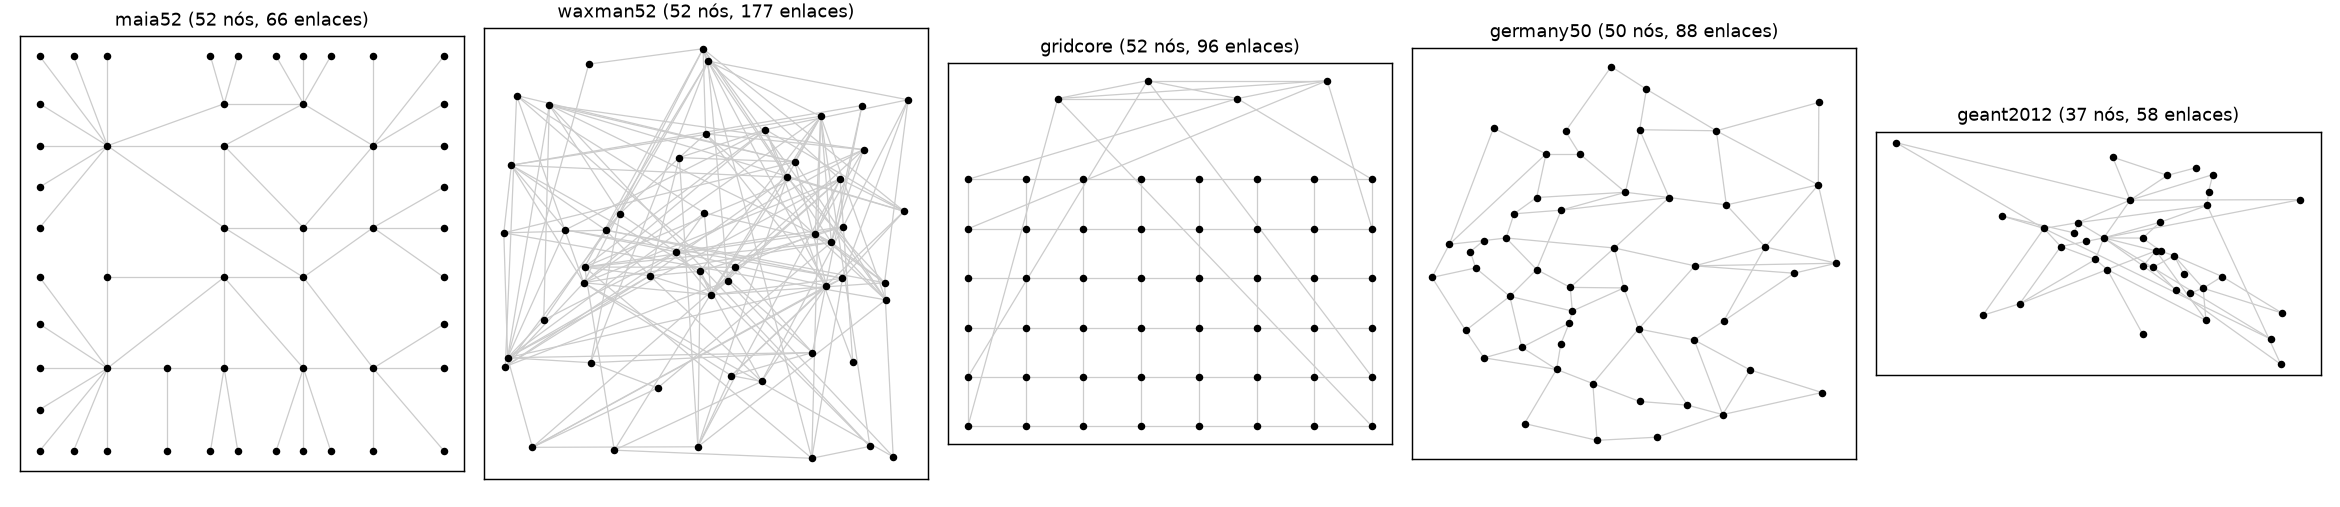
\includegraphics[width=\linewidth]{pt/fig11_topologies.png}
\caption{Instâncias avaliadas: a topologia de estudo original de 52 nós
(maia52), dois grafos sintéticos de 52 nós (waxman52, gridcore) e dois
backbones reais públicos (germany50, geant2012, \emph{marcados real}),
construídos a partir de coordenadas e distâncias de enlace genuínas. Todas
compartilham o mesmo perfil de 17 fluxos e o mesmo ponto de congestão
calibrado.}
\label{fig:topos}
\end{figure}

%=====================================================================
\section{Resultados}
\label{sec:results}

\subsection{Certificação de Otimalidade em Carga Nominal}
\label{sec:cert}
Em carga nominal em maia52, a formulação exata de pool ILP-P certifica o
ótimo do \emph{pool} $\FO=\PoolOptFO$; o ACO$+$AG atinge-o em todas as
replicações (média $\GaFOmaia\pm\GaFOmaiaCI$), igualando o ótimo
certificado, enquanto o ACO$+$DE alcança $\DeFOmaia\pm\DeFOmaiaCI$ e o agente
Q-learning $\QlFOmaia\pm\QlFOmaiaCI$ (Fig.~\ref{fig:cert}). O Dijkstra, que
não otimiza \eqref{eq:fo}, pontua $\DjFOmaia$. O gap de otimalidade do
híbrido em relação ao próprio espaço de busca é, portanto, \emph{zero} ---
propriedade que artigos heurísticos afirmam e raramente demonstram. A
Tabela~\ref{tab:fo} mostra a mesma comparação entre instâncias: com o
\emph{pool} ampliado, o híbrido atinge o ótimo certificado em todas as
instâncias em carga nominal --- nas 20 replicações em maia52, waxman52,
gridcore e germany50, e em 17 de 20 em geant2012 (média \AntGaFO) --- ao
passo que, sem ampliação, o seletor era sensível à seed: antes da ampliação,
o ACO$+$AG chegava a um conjunto factível em apenas metade das replicações
na instância esparsa maia52 (50\% de factibilidade em carga nominal), pois a
diversidade do \emph{pool}, e não o seletor, é a restrição ligante de
designs gerar-e-selecionar. No modelo
revisado, o ILP-L encontra solução factível com utilização máxima mínima
$Z=\IlpZmaia$; CSPF e o híbrido também permanecem factíveis em carga
nominal, mas, sem objetivo de balanceamento, seus perfis de utilização são
piores (Seção~\ref{sec:sweep}).
A Fig.~\ref{fig:conv} mostra a dinâmica de convergência por trás dessas
pontuações, junto com a ablação da semeadura construtiva: sem ampliação do
\emph{pool} (cinza), o mesmo seletor parte $\approx$16 pontos de FO abaixo e
por vezes estagna abaixo do ótimo, enquanto o híbrido ampliado atinge o
ótimo certificado por volta da geração 20 em todas as seeds e permanece
monotonicamente estável depois; nas instâncias mais densas o conjunto ótimo
já está presente desde a primeira geração --- o esforço de convergência
concentra-se justamente onde os limites certificados são mais apertados.

\begin{table}[!t]
\caption{Pontuação da função objetivo em carga nominal (20 seeds, média
$\pm$ IC 95\%). Dijkstra e CSPF são determinísticos.}
\label{tab:fo}
\centering
\begin{tabular}{@{}lrrrrr@{}}
\toprule
Topologia & Dijkstra & CSPF & Q-learn & ACO+DE & ACO+AG\\
\midrule
maia52 & 120 & 132 & 130$\pm$1 & 132$\pm$0 & 132$\pm$0\\
waxman52 & 132 & 132 & 132$\pm$0 & 132$\pm$0 & 132$\pm$0\\
gridcore & 130 & 132 & 132$\pm$0 & 132$\pm$0 & 132$\pm$0\\
germany50 & 128 & 132 & 132$\pm$1 & 132$\pm$0 & 132$\pm$0\\
geant2012 & 128 & 130 & 130$\pm$0 & 130$\pm$0 & 132$\pm$0\\
\bottomrule
\end{tabular}

\end{table}

\begin{figure}[!t]
\centering
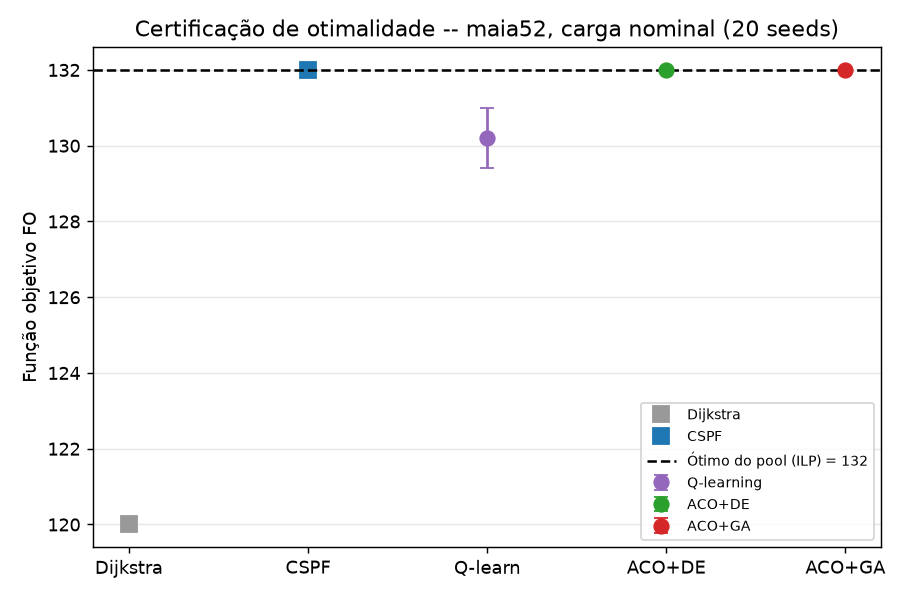
\includegraphics[width=\linewidth]{pt/fig8_optimality.png}
\caption{Pontuação da função objetivo em carga nominal (maia52, 20 seeds,
média $\pm$ IC 95\%). A linha tracejada é o ótimo exato do pool certificado
pelo ILP-P; o ACO+AG atinge-o em todas as replicações.}
\label{fig:cert}
\end{figure}

\begin{figure}[!t]
\centering
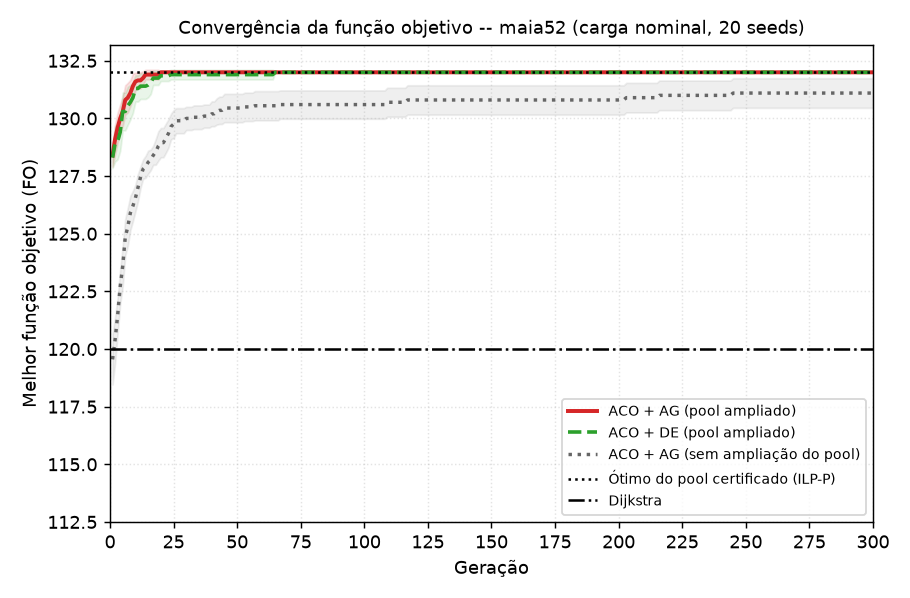
\includegraphics[width=\linewidth]{pt/fig2_convergence.png}
\caption{Convergência da função objetivo em maia52 em carga nominal: melhor
FO por geração, média $\pm$ IC 95\% em 20 seeds. O híbrido com pool
ampliado atinge o ótimo certificado ($\FO=132$) por volta da geração 20 em
todas as seeds e nunca recua abaixo dele; sem ampliação do pool (cinza), o
mesmo seletor parte $\approx$16 pontos de FO abaixo e por vezes estagna
abaixo do ótimo.}
\label{fig:conv}
\end{figure}

\subsection{Varredura de Carga: Certificação Exata do Gargalo sob Stress}
\label{sec:sweep}
O resultado central do modelo exato é o \emph{limite inferior de gargalo}.
A $f=1{,}25$ em maia52, o ILP-L certifica $Z^{*}=\IlpZmaiaHigh$: sob
restrições duras, \emph{nenhum} conjunto de caminhos para os 22 fluxos em
$G$ consegue manter todos os enlaces abaixo de \IlpZmaiaHighPct\% de
utilização --- a instância está demonstravelmente no seu limite, e o limite
certificado quantifica exatamente o quão apertada ela é. A $f=1{,}5$ o
limite \emph{permanece} em $Z^{*}=\IlpZmaiaMax$ em maia52 e
$Z^{*}=\IlpZWaxMax/\IlpZGridMax$ em waxman52/gridcore: mesmo no maior
crescimento testado, um roteamento factível persiste com folga de
$13\%$--$1{,}6\%$ conforme a instância --- e, notavelmente, o próprio
\emph{pool} contém uma combinação plenamente factível a $f=1{,}5$ (ótimo do
pool $\FO=192$ nas 20 replicações), mas o seletor estocástico a atinge em
apenas \GaFeasMaiaMax\% delas. A certificação é o que separa ``o pool é
incompleto'' de ``o seletor falhou'' --- a primeira é falsa aqui, a segunda é
mensurável.
Declaramos também, com honestidade, a limitação do bound: a $f\le 1$ o
valor certificado é dominado pelo maior fluxo individual
($Z^{*}=f\,\lambda_{\max}/\mu$ exatamente, p.ex.\ $0{,}872$ em carga
nominal), pois nenhum roteamento consegue dividir uma única mercadoria; o
conteúdo não trivial do certificado é o regime $f>1$, em que efeitos de
congestão conjunta tornam o bound estritamente maior que qualquer bound de
commodity única. Resoluções exatas lexicográficas levam até poucas dezenas
de segundos (Tabela~\ref{tab:time}), tornando tais certificados práticos
nessa escala.

As heurísticas, em contraste, nunca reportam certificado --- e a dispersão
de qualidade delas é exatamente o que os limites certificados expõem
(Fig.~\ref{fig:viol}, Tabela~\ref{tab:viol}). O Dijkstra, alheio à
capacidade, inflige $\DjViolHigh$ violações de SLA a $f=1{,}25$ e
$\DjViolMax$ a $f=1{,}5$ em maia52, atingindo \DjMaxUtil$\times$ da
capacidade dos enlaces; o CSPF permanece sem violações até $f=1{,}25$, mas
encalha \CspfViolMax\ enlaces sobrecarregados a $f=1{,}5$. O híbrido com
\emph{pool} ampliado permanece sem violações até $f=1{,}25$ e inflige
$\GaViolMax\pm\GaViolMaxCI$ violações a $f=1{,}5$; o agente Q-learning não
ampliado viola seus orçamentos em todas as cargas estressadas
(\QlViolHigh--\QlViolMax). Em waxman52, gridcore e germany50 a ordenação é a
mesma, com apenas o Dijkstra violando (um a três enlaces sobrecarregados a
$f\ge1{,}25$); em geant2012 todo seletor estocástico incorre em pequenas
contagens de violação desde a carga nominal (\GaViolGeantNominal\ para o GA)
--- o regime difícil de backbone real da Seção~\ref{sec:backbone}. Em termos
operacionais: \emph{o modelo exato diz ao operador quanta folga a rede
demonstradamente tem; o híbrido mantém o SLA intacto onde o pool permite ---
até a fronteira certificada e não além; o agente de aprendizado não oferece
garantia nenhuma justamente quando a rede está apertada}.

\begin{table}[!t]
\caption{Violações de SLA (enlaces sobrecarregados $+$ fluxos com atraso em
violação) em maia52: métodos determinísticos como contagens, estocásticos
como média $\pm$ IC 95\% em 20 seeds.}
\label{tab:viol}
\centering
\begin{tabular}{@{}lrrrrr@{}}
\toprule
Carga & Dijkstra & CSPF & Q-learn & ACO+DE & ACO+AG\\
\midrule
1.0$\times$ & 6+0 & 0+0 & 0.9$\pm$0.4 & 0.0$\pm$0.0 & 0.0$\pm$0.0\\
1.25$\times$ & 6+0 & 0+0 & 1.8$\pm$0.7 & 0.2$\pm$0.2 & 0.0$\pm$0.0\\
1.5$\times$ & 9+0 & 4+0 & 1.9$\pm$0.5 & 1.9$\pm$0.4 & 1.1$\pm$0.4\\
\bottomrule
\end{tabular}

\end{table}

\begin{figure}[!t]
\centering
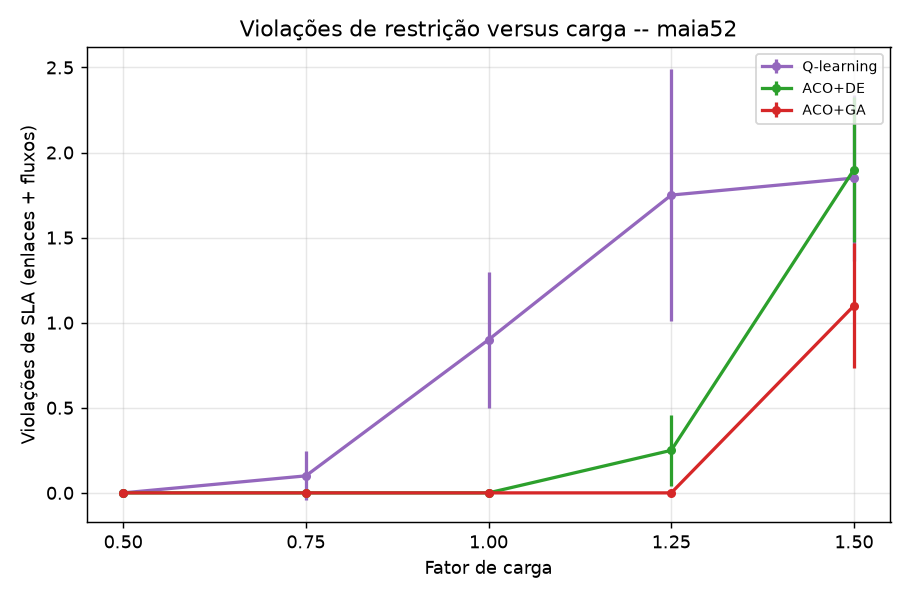
\includegraphics[width=\linewidth]{pt/fig6_violations_maia52.png}
\caption{Violações de SLA (enlaces sobrecarregados $+$ fluxos com atraso em
violação) versus fator de crescimento de sessões em maia52 (média $\pm$ IC
95\% em 20 seeds). O híbrido com pool ampliado permanece sem violações até
$1{,}25\times$; o roteamento de menor caminho degrada primeiro e o agente
Q-learning não oferece garantia de factibilidade.}
\label{fig:viol}
\end{figure}

\subsection{Backbones Reais: um Regime que as Instâncias Sintéticas Escondem}
\label{sec:backbone}
Os dois backbones públicos da Tabela~\ref{tab:topo} carregam geografia
genuína (Seção~\ref{sec:setup}) e se comportam qualitativamente como maia52
--- exceto o \emph{geant2012}, que expõe um regime que as instâncias de 52
nós não mostram. Nessa rede pan-europeia, o baseline construtivo CSPF é
\emph{ele próprio} inviável em carga nominal: ele ultrapassa a capacidade em
um enlace (\AntCspfMaxUtil$\times$ de utilização, \AntCspfViol\ violação)
porque seu compromisso guloso por fluxo esgota um enlace central, e o
Dijkstra é pior (\AntDjMaxUtil$\times$). Essa é exatamente a situação para a
qual o híbrido com \emph{pool} ampliado foi projetado: o ILP-P certifica que
o \emph{pool} contém uma combinação plenamente admissível
($\FO=\AntPoolOpt$) em \AntPoolOptFeasRate\% das replicações, e o híbrido
alcança esse ótimo certificado em \AntGaFeas\% das replicações ---
permanecendo factível onde ambos os baselines gulosos violam, enquanto os
seletores estocásticos alternativos são factíveis em no máximo \AntDeFeas\%
(DE) e \AntQlFeas\% (Q-learning) das replicações (Tabela~\ref{tab:backbone}). O
modelo exato min--max certifica $Z^{*}=\GeantZ$ em carga nominal --- deixando
$100(1-\GeantZ)\%$ de folga que nenhum roteamento naquela carga consegue
exceder, uma garantia que as heurísticas não produzem.

Dois achados dependentes de regime merecem destaque. Primeiro, a restrição
\emph{dura} de atraso é ativa nas instâncias sintéticas de alta latência
(maia52, enlaces de 1--80~ms) mas \emph{frouxa} nos backbones reais, cuja
propagação em fibra é \AntDelayGeantMin--\AntDelayGeantMax\,ms --- bem abaixo
do orçamento de 150~ms --- de modo que a discriminação lá vem apenas da
restrição de capacidade. Isso é fisicamente fiel: violações reais de SLA
fim-a-fim são impulsionadas por fila, não por propagação, exatamente o que a
simulação a nível de pacotes da Seção~\ref{sec:qos} captura. Segundo, o
benefício de plano de dados do SRv6 (Seção~\ref{sec:srv6res}) acompanha o
comprimento médio do caminho: os caminhos mais curtos dos backbones produzem
reduções menores, embora ainda substanciais (\SrvRedGer$\times$ e
\SrvRedGeant$\times$), do que os grafos sintéticos de alta latência
(\SrvRedMaia$\times$), porque o número de regras por fluxo é proporcional aos
saltos do caminho, não à geografia.

\begin{table}[!t]
\caption{Resultados de backbone real em carga nominal (20 seeds, média
$\pm$ IC 95\% salvo determinísticos). O ILP-P certifica o ótimo do pool; o
ILP-L certifica o limite exato de gargalo.}
\label{tab:backbone}
\centering
\begin{tabular}{@{}lrrrr@{}}
\toprule
Método & FO & Factível & Util. máx. & Observação\\
\midrule
Dijkstra & \AntDjFO & --- & \AntDjMaxUtil & determinístico\\
CSPF & \AntCspfFO & --- & \AntCspfMaxUtil & construtivo\\
ACO$+$AG (ampl.) & \AntGaFO & \AntGaFeas\% & --- & este trabalho\\
ACO$+$DE (ampl.) & \AntDeFO & \AntDeFeas\% & --- & este trabalho\\
Q-learning & \AntQlFO & \AntQlFeas\% & --- & tabular\\
ILP-P (pool) & \AntPoolOpt & --- & --- & certificado\\
ILP-L (MCF) & --- & --- & \GeantZ & certificado $Z^{*}$\\
\bottomrule
\end{tabular}
\end{table}

\subsection{Qualidade de Balanceamento}
A Fig.~\ref{fig:maxutil} reporta a utilização máxima de enlace em maia52. Em
carga nominal o ótimo exato min--max é $Z=\IlpZmaia$; CSPF e o híbrido
permanecem próximos do limite de capacidade ($Z\approx 1{,}0$), mas acima do
valor exato, e o Dijkstra excede a capacidade completamente
($Z\approx\DjMaxUtil$). À medida que a carga passa da fronteira de
factibilidade, a comparação via utilização deixa de ser significativa (todos
os métodos excedem a capacidade); a contagem de violações da
Seção~\ref{sec:sweep} passa a carregar o sinal operacional.

\begin{figure}[!t]
\centering
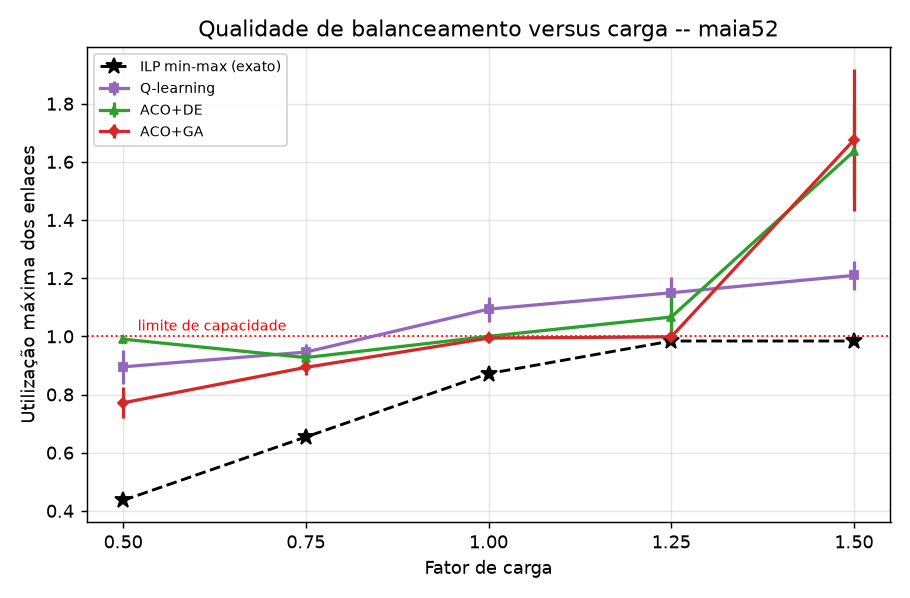
\includegraphics[width=\linewidth]{pt/fig7_maxutil_maia52.png}
\caption{Utilização máxima de enlace versus carga (maia52). A utilização
min--max exata do modelo revisado (ILP-L) é a linha de referência; a
factibilidade termina na fronteira certificada.}
\label{fig:maxutil}
\end{figure}

\subsection{QoS a Nível de Pacote em Condições Idênticas}
\label{sec:qos}
Com filas idênticas, capacidades por par de enlace compartilhadas entre os
dois sentidos (mesma convenção do otimizador) e taxas de injeção idênticas,
o roteamento otimizado sustenta \SimThrGain\ mais de boa-vazão entregue
média que o Dijkstra e reduz o atraso fim-a-fim médio de \SimDelayDj~ms
para \SimDelayOpt~ms e a perda por admissão (drops) de \SimLossDj\% para
\SimLossOpt\%; o jitter estilo RFC 3550 cai apenas de \SimJitDj~ms para
\SimJitOpt~ms --- mudança modesta que reportamos sem enfeite, pois pacotes
sobreviventes de um fluxo com perdas podem carregar jitter baixo.
Convenções: ``perda'' conta apenas drops de admissão (pacotes ainda em
voo no fim da janela não são entregues nem contados como perdidos),
``jitter'' é a variação absoluta média de atraso entre pacotes consecutivos
(estilo RFC 3550, \emph{não} o estimador do D-ITG) e a boa-vazão é bits
entregues na janela. O simulador é determinístico dado o roteamento e o
cronograma de injeção (sem elementos estocásticos), de modo que reportamos
valores de realização única; toda a variabilidade amostral vive na camada de
cálculo de rotas, onde é replicada e testada (Seção~\ref{sec:sweep}). A
simulação controlada reproduz a \emph{direção} dos resultados da bancada
emulada do estudo original com magnitudes moderadas; a
Seção~\ref{sec:bench} explica por que as magnitudes da bancada são
maiores.

\begin{figure}[!t]
\centering
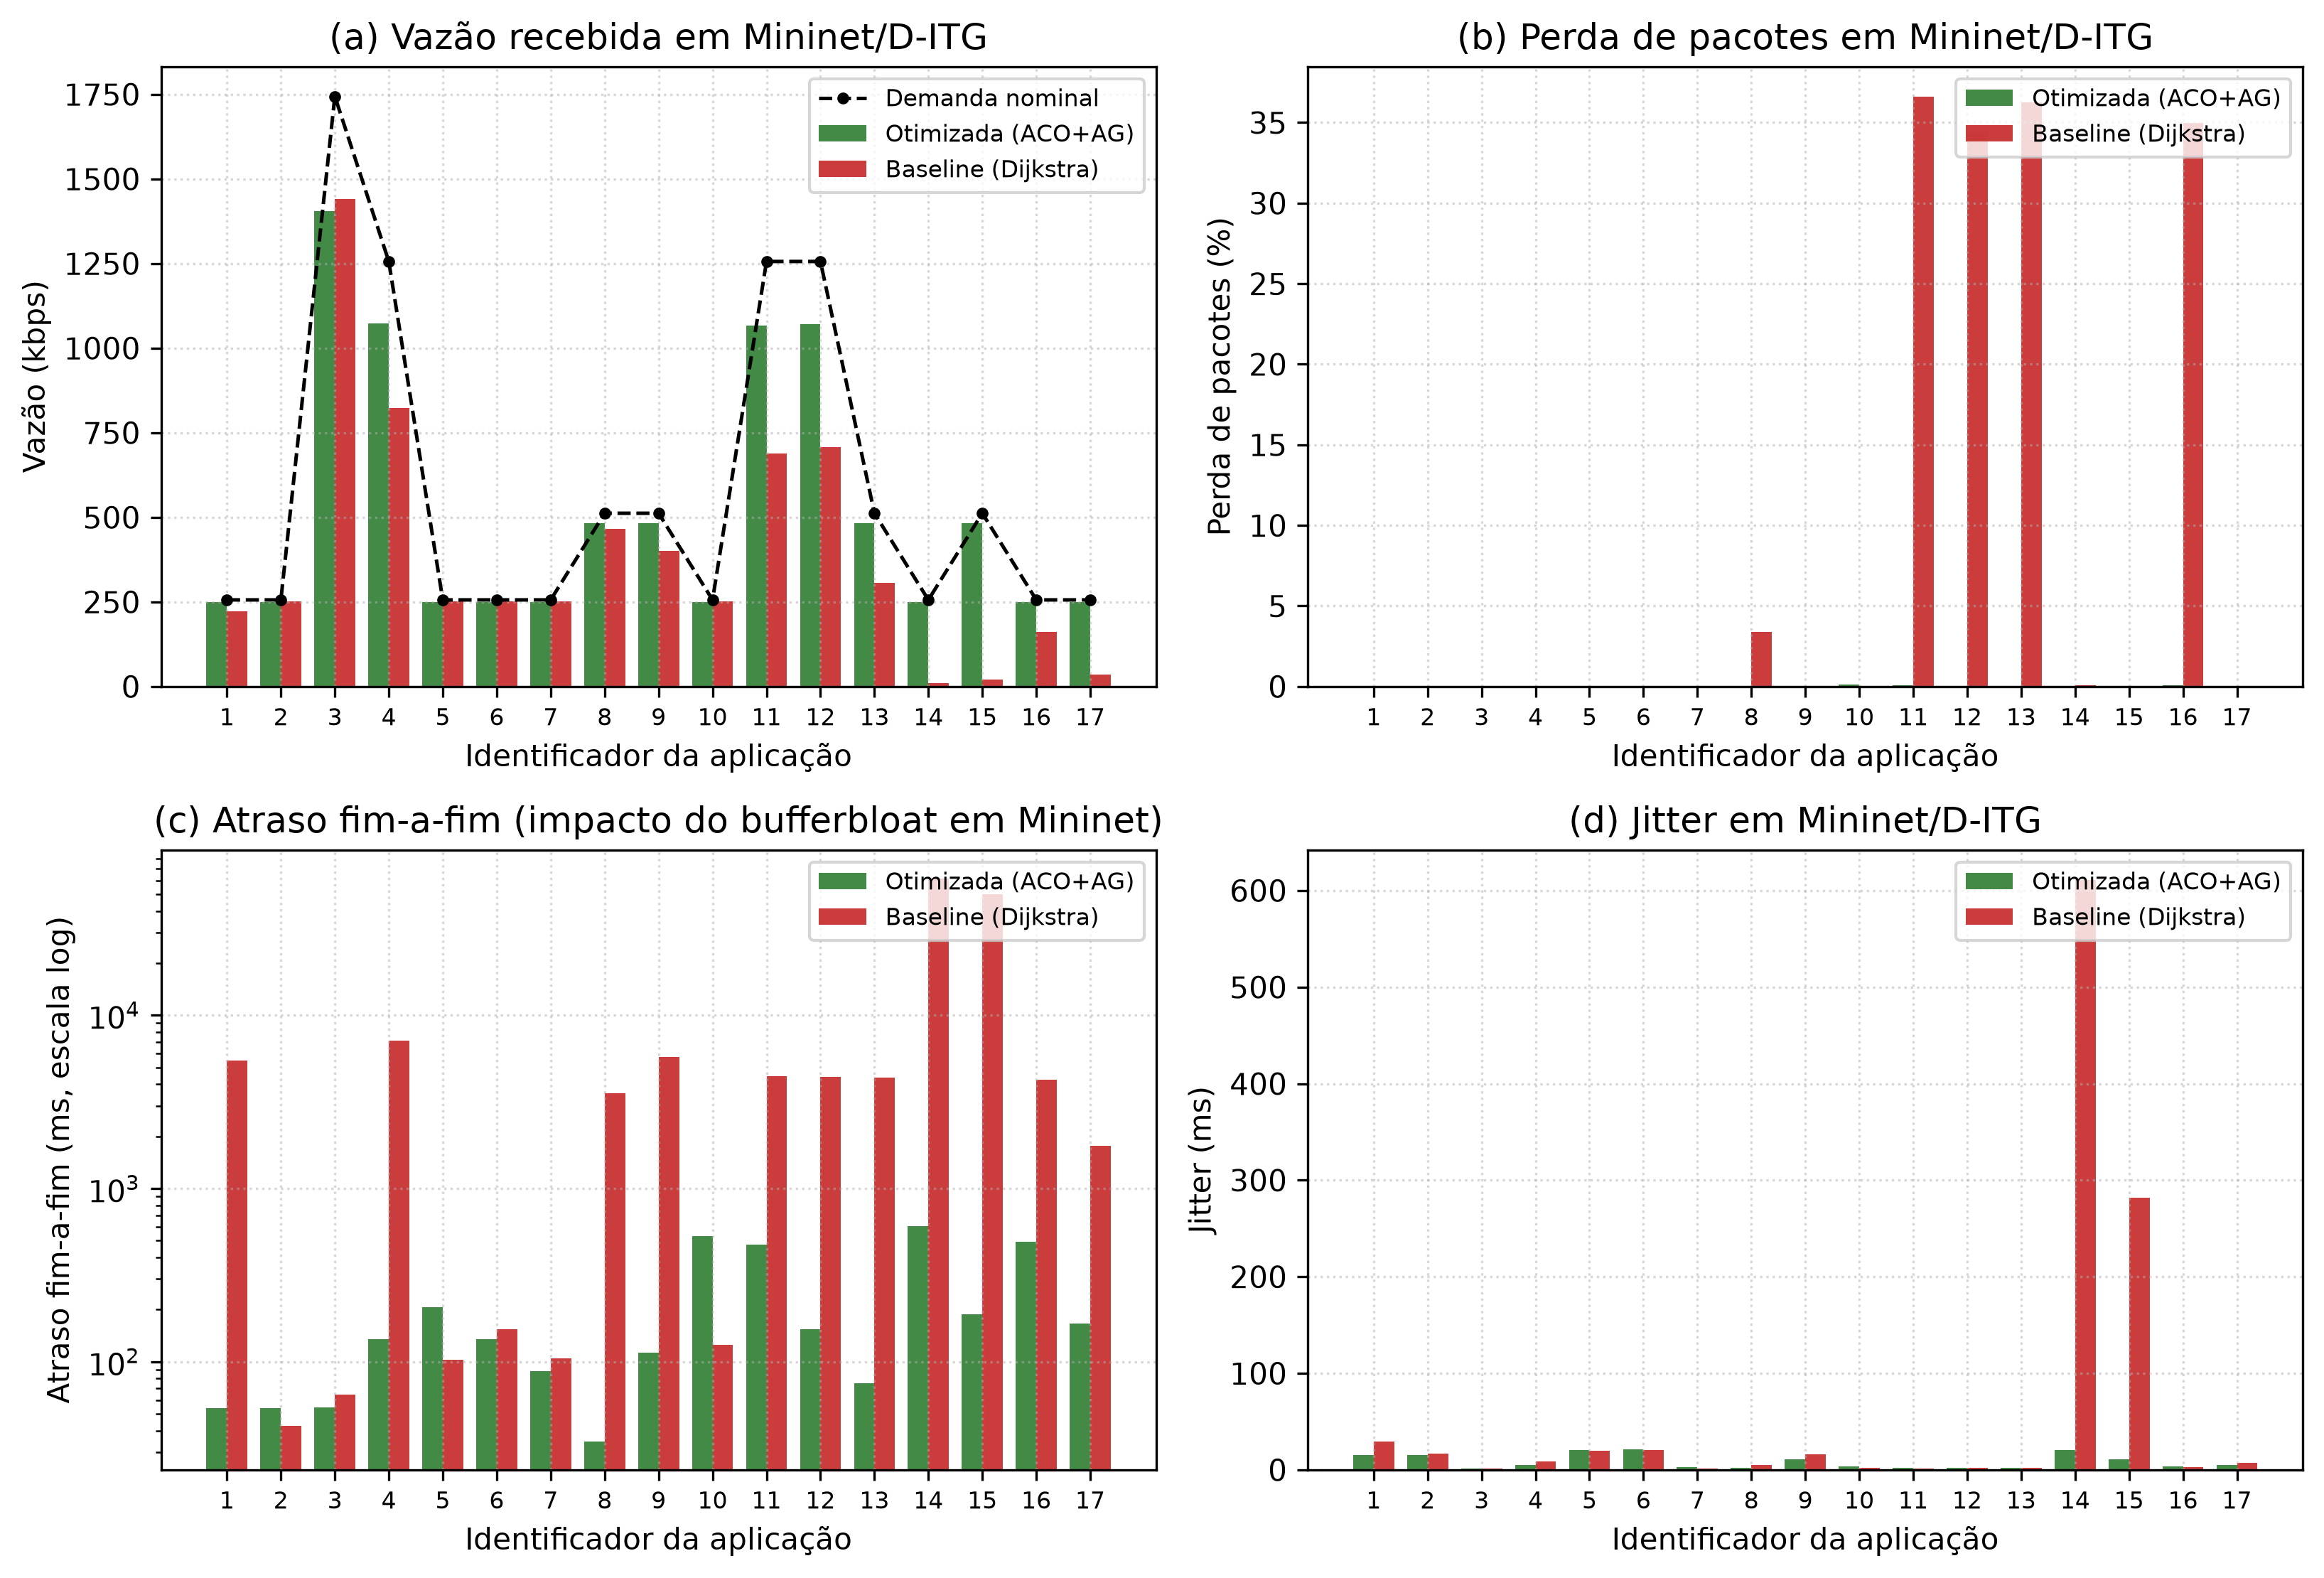
\includegraphics[width=\linewidth]{pt/fig3_mininet_results.png}
\caption{Bancada emulada (Mininet/Floodlight/D-ITG): vazão, perda, atraso e
jitter por aplicação, roteamento otimizado versus menor caminho (dados do
estudo original). A direção de todos os efeitos coincide com a simulação
controlada; as magnitudes diferem (Seção~\ref{sec:bench}).}
\label{fig:mininet}
\end{figure}

\subsection{Diferenciação Lógica sob Amplificação do Fundo}
\label{sec:slicesres}
Medimos fluxos sensíveis a atraso (as quatro aplicações mapeadas à classe
URLLC na Tabela~\ref{tab:apps}; 150~ms é um orçamento experimental deste
estudo, não uma definição 3GPP de URLLC) à taxa nominal enquanto o fundo
eMBB/mMTC é amplificado de $1\times$ a $4\times$, tanto na instância de
estudo quanto no backbone alemão real. No \emph{germany50}
(Fig.~\ref{fig:slices-ger}) o efeito é limpo e fisicamente realista: com
roteamento otimizado, os fluxos prioritários mantêm \GerDoptOne~ms a
$1\times$ e \GerDoptTwo~ms a $2\times$ com \GerLossOptTwo\% de perda,
degradando para \GerDoptThree~ms a $3\times$ --- cruzando o orçamento
experimental --- enquanto o roteamento por menor caminho colapsa para
\GerDdjTwo~ms e \GerLossDjTwo\% de perda já em carga nominal: o baseline não
consegue proteger os fluxos prioritários em nenhum nível. Na instância de
estudo de alta latência \emph{maia52} (Fig.~\ref{fig:slices}), o contraste é
ainda mais forte: o roteamento otimizado mantém os fluxos prioritários em
\UrllcDoptFifteen~ms a $1{,}5\times$ e cruza o orçamento a $2\times$
(\UrllcDoptTwo~ms), enquanto o roteamento por menor caminho viola o
orçamento em \emph{todos} os níveis (\UrllcDdjOne~ms já a $1\times$) e perde
até \UrllcLossDjFour\% a $4\times$. Declaramos deliberadamente que isto não
é isolamento de fatia: a restrição de capacidade é agregada sobre todas as
fatias em cada enlace e todas as filas são FIFO --- o que a estrutura de
restrições entrega é diferenciação determinística, ordenada por prioridade,
sob capacidade compartilhada (os fluxos prioritários degradam por último e
menos), não o isolamento garantido de uma partição dedicada. O caso do
backbone real mostra esse mecanismo com latências realistas de sub-2~ms.

\begin{figure*}[!t]
\centering
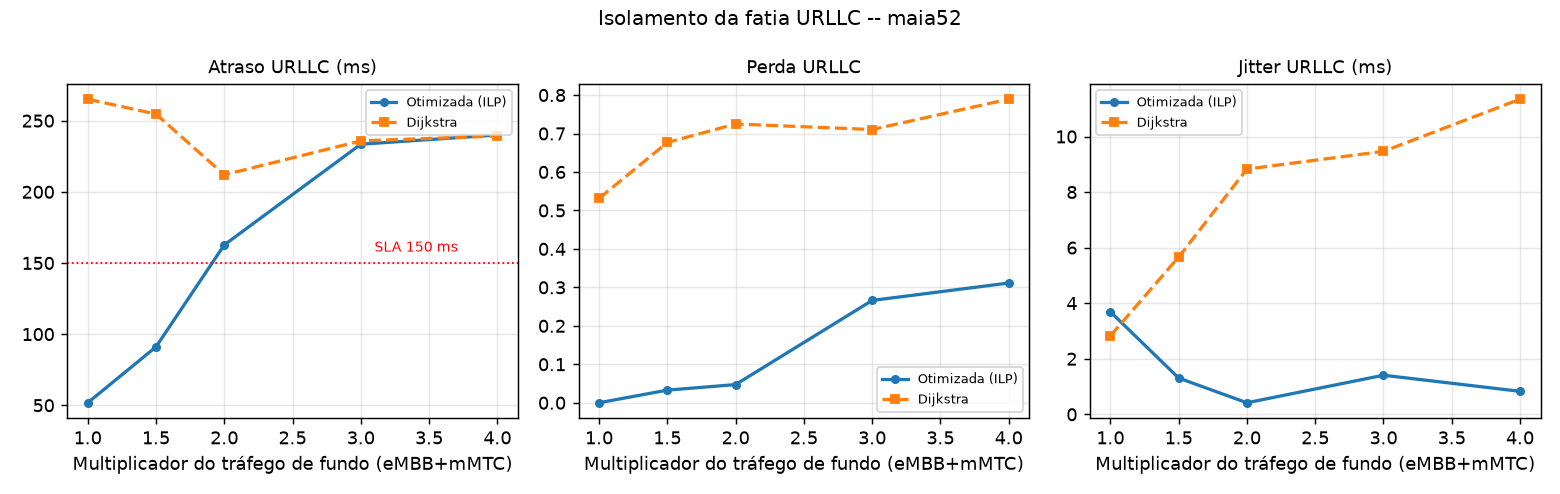
\includegraphics[width=0.92\textwidth]{pt/fig10_slice_isolation.png}
\caption{Fluxos sensíveis a atraso (mapeados à classe URLLC; orçamento
experimental de 150~ms) sob amplificação crescente do fundo eMBB/mMTC na
instância de estudo \emph{maia52}, roteamento otimizado versus menor
caminho.}
\label{fig:slices}
\end{figure*}

\begin{figure*}[!t]
\centering
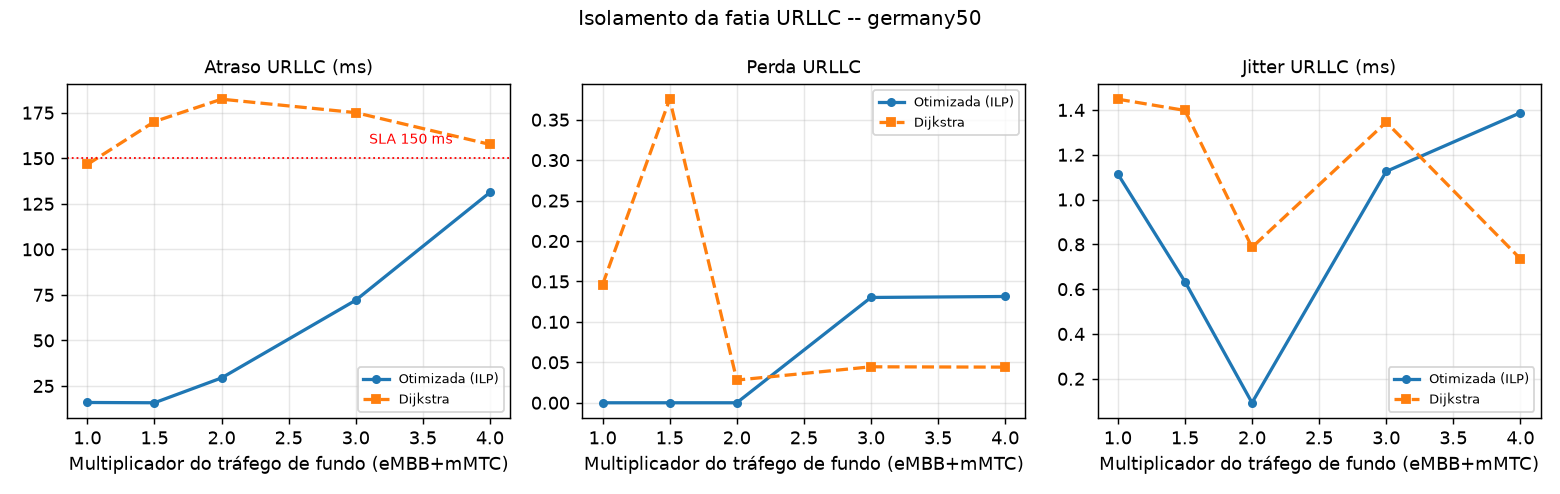
\includegraphics[width=0.92\textwidth]{pt/fig10_germany50_slice_isolation.png}
\caption{Diferenciação lógica de fluxos sensíveis a atraso (mapeados à
classe URLLC) no backbone real de pesquisa alemão (\emph{germany50}), com
latências realistas de sub-2~ms. O roteamento otimizado mantém os fluxos
prioritários em $\sim\GerDoptTwo$~ms e $\GerLossOptTwo\%$ de perda até
$2\times$ de fundo, enquanto o roteamento por menor caminho degrada para
$\sim\GerDdjTwo$~ms e $\GerLossDjTwo\%$ de perda já em carga nominal.}
\label{fig:slices-ger}
\end{figure*}

\subsection{Contabilidade de Estado SRv6 Calculada}
\label{sec:srv6res}
A Tabela~\ref{tab:srv6} e a Fig.~\ref{fig:srv6} reportam o estado do plano
de dados calculado (contabilidade analítica sobre os caminhos produzidos;
não há medição de TCAM nem execução em hardware). Codificar as mesmas rotas otimizadas como listas de
segmentos SRv6 exige exatamente uma regra por fluxo no seu \emph{headend}
(\SrvSrRules\ regras para 17 fluxos) e \emph{zero} estado por fluxo nos nós
de trânsito, contra \SrvOfMaia--\SrvOfGrid\ regras OpenFlow por fluxo
distribuídas pelos comutadores de trânsito nas cinco instâncias ---
reduções medidas de \SrvRedMaia$\times$ (maia52), \SrvRedWax$\times$
(waxman52), \SrvRedGrid$\times$ (gridcore), \SrvRedGer$\times$ (germany50) e
\SrvRedGeant$\times$ (geant2012). A maior lista de segmentos tem
\MaxSLAll\ SIDs (gridcore) --- acima dos limites de lista de segmentos
comumente suportados por hardware de encaminhamento (tipicamente 6--8 SIDs),
o que na prática exigiria compressão uSID/G-SID --- e gera custo máximo
calculado de encapsulamento de \MaxSrhBytes\ bytes por pacote; os backbones,
com caminhos mais curtos, produzem reduções menores porém ainda substanciais
(\SrvRedGer$\times$--\SrvRedGeant$\times$), pois a redução acompanha o
comprimento médio do caminho em saltos. Duas ressalvas delimitam a
afirmação: primeiro, a redução é calculada contra o \emph{pior caso} da
programação OpenFlow (uma regra por fluxo em cada comutador de trânsito);
regras agregadas, rótulos MPLS ou túneis reduziriam o gap. Segundo, a
contabilidade conta regras, não bits de TCAM, latência de programação nem
overhead de encaminhamento do SRH --- é uma afirmação de pegada de estado,
não de desempenho. O efeito é estrutural: vale para toda filosofia de
roteamento calculada (Dijkstra, CSPF e o otimizador), pois move o estado do
caminho da rede para o pacote.

\begin{figure}[!t]
\centering
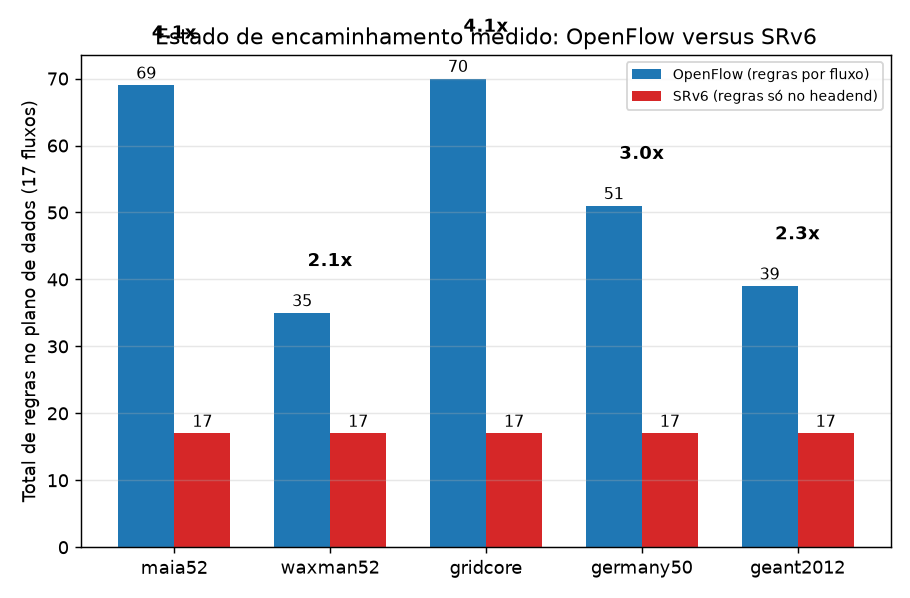
\includegraphics[width=\linewidth]{pt/fig9_srv6_state.png}
\caption{Estado de encaminhamento medido para o mesmo roteamento de 17
fluxos sob programação OpenFlow por fluxo versus programação SRv6 somente no
headend.}
\label{fig:srv6}
\end{figure}

\begin{table}[!t]
\caption{Estado do plano de dados medido (roteamento CSPF, 17 fluxos).}
\label{tab:srv6}
\centering
\begin{tabular}{@{}lrrrrr@{}}
\toprule
Topologia & Regras OF & Máx/nó OF & Regras SRv6 & Máx SIDs & Redução\\
\midrule
maia52 & 69 & 9 & 17 & 6 & 4.1$\times$\\
waxman52 & 35 & 4 & 17 & 4 & 2.1$\times$\\
gridcore & 70 & 4 & 17 & 10 & 4.1$\times$\\
germany50 & 51 & 5 & 17 & 6 & 3.0$\times$\\
geant2012 & 39 & 6 & 17 & 8 & 2.3$\times$\\
\bottomrule
\end{tabular}

\end{table}

\subsection{Baseline de Aprendizado sob o Mesmo Protocolo}
\label{sec:qlb}
O agente Q-learning tabular alcança $\QlFOmaia\pm\QlFOmaiaCI$ em carga
nominal em maia52 --- próximo do ótimo certificado --- mas sua factibilidade
é sensível à instância e à seed: na maia52 esparsa ele monta um conjunto de
rotas sem violações em apenas \QlFeasNominal\% das replicações em carga
nominal, e sob stress inflige $\QlViolHigh$ violações a $f=1{,}25$ contra
$\GaViolHigh$ do ACO$+$AG (Wilcoxon $p=\QlVsGaP$), enquanto nas instâncias
sintéticas mais densas iguala o ótimo certificado em toda a varredura. Seu
treinamento por cenário ($\QlTime$~s) é gasto novamente a cada nova época de
tráfego, enquanto a meta-heurística recalcula a partir do estado
instantâneo ($\GaTime$~s). Declaramos o escopo dessa evidência com precisão: ela
concerne \emph{este agente tabular sob este protocolo}, não roteadores DRL
modernos (políticas baseadas em GNN, TE multi-agente), que podem fechar
parte dessas lacunas
\cite{xu2018experience,stampa2017drl,almasan2022drl}. O que o experimento
estabelece é estrutural: um seletor orientado a recompensa sem modelo de
restrições não fornece certificado de factibilidade e, no nosso protocolo,
paga custo de amostragem por cenário. Posicionamos, portanto, a otimização
com restrições explícitas --- estocástica onde a escala exige, exata onde é
acessível --- como núcleo de decisão, com aprendizado como preditor a
montante, não como substituto.

\subsection{Tempo de Execução}
Todos os métodos são rápidos o suficiente para épocas de TE off-line
(Tabela~\ref{tab:time}): o ILP exato de pool resolve em $\PoolTime$~s, o ILP
exato de enlaces em $\IlpTime$~s, uma execução do híbrido em $\GaTime$~s, e
o Q-learning em $\QlTime$~s por cenário em CPU de classe desktop --- ou
seja, o custo de otimização não é o gargalo operacional nessa escala; o que
distingue os métodos é o valor da certificação.

\begin{table}[!t]
\caption{Tempo de relógio mediano por decisão completa de roteamento (s).}
\label{tab:time}
\centering
\begin{tabular}{@{}lrr@{}}
\toprule
Método & Tempo mediano (s) & Modelo\\
\midrule
Dijkstra & 0.0 & determinístico\\
CSPF & 0.0 & determinístico\\
ACO+AG & 6.8 & estocástico\\
ACO+DE & 5.1 & estocástico\\
Q-learning & 0.2 & aprendizado\\
ILP-P (pool) & 0.1 & exato\\
ILP-L (MCF) & 0.6 & exato\\
\bottomrule
\end{tabular}

\end{table}

\subsection{Reconciliando Simulação e Emulação}
\label{sec:bench}
A simulação controlada e a bancada emulada concordam na direção de todos os
efeitos, mas diferem em magnitude: a bancada reporta razões de $51\times$
(atraso) e $510\times$ (perda) contra o roteamento por menor caminho,
enquanto a simulação controlada reporta razão de atraso de
\SimDelayRatio$\times$ e \emph{eliminação} dos drops de admissão
(\SimLossOpt\% vs.\ \SimLossDj\%), o que torna a razão de perda indefinida,
não grande. A explicação está no baseline, não no otimizador: com
roteamento por menor caminho por fluxo, um enlace gargalo de 2~Mbps
carregando vários fluxos nominais desenvolve uma fila profunda persistente
(\emph{bufferbloat}; 10,8~s de atraso de fila medidos na bancada). A
magnitude da melhoria depende, portanto, primariamente do dimensionamento e
do gerenciamento de fila do deployment do baseline --- um artefato de
configuração --- e não do otimizador em si. Reportamos a simulação
controlada com buffers fixos e modestos (80 pacotes) como referência
reproduzível, e a bancada como confirmação qualitativa; desencorajamos
explicitamente citar razões entre configurações sem declarar a configuração
de fila.

%=====================================================================
\section{Ameaças à Validade e Limitações}
\label{sec:limits}
\textbf{Escala e capacidade de enlace.} As instâncias abrangem 37--52 nós e
17--27 fluxos. Duas delas são backbones reais, o que fortalece a validade
externa, mas não alcança a escala de operadora ou de Internet. Os arquivos
GML públicos desses backbones não trazem capacidade por enlace, portanto ---
como declarado na Seção~\ref{sec:setup} --- aplicamos uma calibração fixa
para colocar cada instância no mesmo ponto de congestão certificado
($Z^{*}=0{,}87$ em carga nominal). Os valores absolutos de capacidade são,
assim, um controle experimental, não uma afirmação sobre largura de banda
real provisionada; todas as afirmações comparativas (qual método é factível,
qual é melhor) são invariantes a essa escolha porque cada método é avaliado
na instância idêntica. Capacidades reais heterogêneas por enlace permanecem
trabalho futuro. As formulações ILP
escalam com $|E|\,L$ variáveis binárias e foram resolvidas em segundos aqui;
instâncias maiores exigiriam decomposição ou geração de colunas.
\textbf{Modelo de atraso apenas por propagação.} O atraso fim-a-fim nos
experimentos combinatórios é propagação mais um termo fixo por salto; o
atraso de fila surge apenas na simulação a nível de pacotes. É por isso que a
restrição dura de atraso é ativa nas instâncias sintéticas de alta latência e
frouxa nos backbones reais, e significa que a restrição de capacidade --- não
o orçamento de atraso --- é a que vincula em topologias realistas. Modelar o
atraso de fila dentro do ILP (uma extensão de redes estocásticas) é um passo
natural a seguir.
\textbf{Modelo de tráfego.} A injeção a taxa constante (estilo UDP) abstrai
a dinâmica do TCP; cargas TCP com controle de congestionamento podem
deslocar a fronteira de violações e ficam para trabalho futuro. A evidência
de bancada (D-ITG) carrega a mesma abstração.
\textbf{Rótulos de crescimento de carga.} Os fatores ``$1{,}25\times$'' e
``$1{,}5\times$'' são parâmetros de crescimento de sessões; o tráfego
oferecido agregado correspondente é \LoadRatioHigh$\times$ e
\LoadRatioMax$\times$ o nominal (Seção~\ref{sec:setup}). Eixos que os
plotam como ``fator de carga'' linear devem ser lidos com isso em mente.
\textbf{Tolerância da certificação.} O limite de gargalo é certificado por
resolução lexicográfica em duas fases ($Z$ mínimo, depois desempate por
atraso com $Z$ fixado a $10^{-6}$); todas as fases aqui terminam Optimal,
mas em escala maior o limite de tempo da fase 1 exigiria gap de otimalidade
declarado. A $f\le 1$ o bound certificado é dominado pelo maior fluxo
individual ($Z^{*}=f\,\lambda_{\max}/\mu$), e seu conteúdo é o regime
$f>1$ (Seção~\ref{sec:sweep}).
\textbf{Convenções do simulador.} A perda conta apenas drops de admissão
(pacotes em voo excluídos); o jitter é o estimador estilo RFC 3550
(variação absoluta média entre pacotes consecutivos), não o do D-ITG; a
capacidade é compartilhada por par não direcionado, como no otimizador.
Essas convenções diferem da bancada do estudo original e do rascunho
anterior deste artigo; todos os números a nível de pacote desta versão as
seguem.
\textbf{Reutilização do pool.} Os \emph{pools} candidatos são gerados em
carga nominal e reutilizados na varredura; um \emph{pool} adaptativo à carga
poderia deslocar levemente a fronteira, embora a diversidade do pool seja
guiada pela topologia. Na carga mais apertada ($f=1{,}5$ em maia52), o pool
certifica conter um conjunto factível, mas o seletor estocástico nem sempre
o encontra --- limitação honesta do estágio de seleção que o modelo exato
fecha.
\textbf{Pesos do objetivo.} O modelo de pontuação retém pesos arbitrários por
desígnio (continuidade com a formulação original); todas as conclusões de
factibilidade e balanceamento são extraídas do modelo revisado, que é isento
de pesos.
\textbf{Demandas estáticas.} O modelo otimiza um retrato; re-otimização
reativa sob churn e interação com controle de admissão são problemas de
engenharia em aberto.

%=====================================================================
\section{Conclusão}
\label{sec:conc}
Reformulamos a engenharia de tráfego com QoS para SDN separando dois
modelos --- o escore de admissão original, que o híbrido otimiza, e uma
formulação revisada de restrições duras com objetivo min--max, que resolvemos
exatamente e lexicograficamente --- e usamos as soluções exatas para
certificar, não afirmar, a qualidade de um híbrido em dois estágios (pool ACO
$+$ seleção AG/DE) em cinco instâncias (duas delas backbones reais), cinco
fatores de crescimento de sessões e vinte replicações. Os certificados
sustentam quatro conclusões concretas. O híbrido atinge o ótimo certificado
do seu pool em carga nominal em todas as instâncias (17/20 replicações na
mais difícil), e nunca pontua abaixo do baseline construtivo CSPF por
construção. O modelo exato prova onde a folga da rede termina: todo
roteamento a $1{,}25\times$ de crescimento de sessões na instância esparsa
excede \IlpZmaiaHighPct\% de utilização em algum enlace, enquanto um
roteamento factível persiste com folga de $1{,}6\%$ a $1{,}5\times$ --- mas
o seletor estocástico o encontra em apenas \GaFeasMaiaMax\% das replicações,
um limite mensurável de designs gerar-e-selecionar sob stress. No GEANT o
baseline construtivo é ele próprio inviável e o híbrido permanece factível
em \AntGaFeas\% das replicações. A simulação a nível de pacotes com
capacidades compartilhadas por par mostra diferenciação ordenada por
prioridade --- fluxos sensíveis a atraso degradam por último e menos --- em
vez de isolamento garantido. Por fim, a contabilidade SRv6 calculada limita a
redução de estado de encaminhamento a $2{,}1$--$4{,}1\times$ com comutadores
de trânsito sem estado, sujeita aos limites de hardware de listas de
segmentos. O resultado é um núcleo de engenharia de tráfego auditável para
controladores SDN: exato onde a exatidão é acessível, heurístico onde a
escala exige, e certificado onde quer que seja possível.

\section*{Reprodutibilidade}
Todos os experimentos são produzidos por scripts com seeds fixas (geração de
topologias, pools ACO, meta-heurísticas, baseline Q-learning, modelos ILP
exatos, simulação a nível de pacote, estatística e figuras) liberados com
este artigo; cada número do texto é injetado dos arquivos de resultados
gerados.

%=====================================================================
\begin{thebibliography}{30}

\bibitem{mckeown2008} N. McKeown \emph{et al.}, ``OpenFlow: Enabling
innovation in campus networks,'' \emph{ACM SIGCOMM Computer Communication
Review}, vol. 38, no. 2, pp. 69--74, 2008.

\bibitem{kim2013} H. Kim and N. Feamster, ``Improving network management with
software defined networking,'' \emph{IEEE Communications Magazine}, vol. 51,
no. 2, pp. 114--119, 2013.

\bibitem{hu2014} F. Hu, Q. Hao, and M. Bao, ``A survey on software-defined
network and OpenFlow: From concept to implementation,'' \emph{IEEE
Communications Surveys \& Tutorials}, vol. 16, no. 4, pp. 2181--2206, 2014.

\bibitem{bosshart2014} P. Bosshart \emph{et al.}, ``P4: Programming
protocol-independent packet processors,'' \emph{ACM SIGCOMM Computer
Communication Review}, vol. 44, no. 3, pp. 87--95, 2014.

\bibitem{dorigo2004} M. Dorigo and T. St\"utzle, \emph{Ant Colony
Optimization}. MIT Press, 2004.

\bibitem{waxman1988} B. M. Waxman, ``Routing of multipoint connections,''
\emph{IEEE Journal on Selected Areas in Communications}, vol. 6, no. 9,
pp. 1617--1622, 1988.

\bibitem{dicaro1998} G. Di Caro and M. Dorigo, ``AntNet: Distributed
stigmergetic control for communications networks,'' \emph{Journal of
Artificial Intelligence Research}, vol. 9, pp. 317--365, 1998.

\bibitem{awduche2002} D. Awduche \emph{et al.}, ``Overview and principles of
Internet traffic engineering,'' IETF RFC 3272, maio 2002.

\bibitem{fortz2000} B. Fortz and M. Thorup, ``Internet traffic engineering by
optimizing OSPF weights,'' in \emph{Proc. IEEE INFOCOM}, 2000,
pp. 519--528.

\bibitem{jain2013} S. Jain \emph{et al.}, ``B4: Experience with a
globally-deployed software defined WAN,'' in \emph{Proc. ACM SIGCOMM},
2013, pp. 3--14.

\bibitem{topozoo} The Internet Topology Zoo: a curated archive of real-world
network topologies, \emph{online}, jul. 2022. [Online]. Disponível em:
http://www.topology-zoo.org

\bibitem{sndlib2016} S. Orlowski and M. Janiak, ``SNDlib --- a library for
designing multi-instance network design problems,'' Relatório Técnico
TR-11-01, Networks Laboratory, Universidade de Wroc\l aw, Polônia, 2011.

\bibitem{xu2018experience} H. Xu, Z. Li, L. Zhou, Z. Li, K. Wang, and Y.
Guo, ``Experience-driven networking: A deep reinforcement learning based
approach,'' in \emph{Proc. IEEE INFOCOM}, 2018, pp. 1871--1879.

\bibitem{stampa2017drl} A. Stampa, M. Arias, D. S\'anchez-Charles, P.
Barlet-Ros, and A. Cabellos-Aparicio, ``A deep-reinforcement learning
approach for software-defined networking routing optimization,'' arXiv
preprint arXiv:1709.07080, 2017.

\bibitem{almasan2022drl} P. Almasan, J. Su\'arez-Varela, A. Badia-Samper, P.
Barlet-Ros, and A. Cabellos-Aparicio, ``Towards deep reinforcement learning
for traffic engineering in SDN,'' \emph{Computer Networks}, vol. 213, art.
109035, 2022.

\bibitem{rfc8402} C. Filsfils, S. Previdi, L. Ginsberg, B. Decraene, S.
Litkowski, and R. Shakir, ``Segment Routing Architecture,'' IETF RFC 8402,
Jul. 2018.

\bibitem{rfc8754} C. Filsfils, D. Dukes, S. Previdi, J. Leddy, S.
Matsushima, and D. Voyer, ``IPv6 Segment Routing Header (SRH),'' IETF RFC
8754, Mar. 2020.

\bibitem{rfc8986} C. Filsfils, P. Camarillo, J. Leddy, D. Voyer, B.
Bernier, and J. Linkova, ``Segment Routing over IPv6 (SRv6) Network
Programming,'' IETF RFC 8986, Feb. 2021.

\bibitem{rfc9256} C. Filsfils, K. Talaulikar, D. Voyer, A. Bogdanov, and P.
Mattes, ``Segment Routing Policy Architecture,'' IETF RFC 9256, Jul. 2022.

\bibitem{rfc4655} A. Farrel, J.-P. Vasseur, and J. Ash, ``A Path Computation
Element (PCE)-Based Architecture,'' IETF RFC 4655, Aug. 2006.

\bibitem{itu-m2083} ITU-R, ``IMT Vision --- Framework and overall objectives
of the future development of IMT for 2020 and beyond,'' Recommendation
ITU-R M.2083-0, Sep. 2015.

\bibitem{3gpp-ts23501} 3GPP, ``System architecture for the 5G System
(5GS),'' Technical Specification TS 23.501, Release 17, 2022.

\bibitem{lantz2010} B. Lantz, B. Heller, and N. McKeown, ``A network in a
laptop: Rapid prototyping for software-defined networks,'' in \emph{Proc.
ACM HotNets}, 2010.

\bibitem{botta2012} A. Botta, A. Dainotti, and A. Pescap\'e, ``On the
validation of D-ITG,'' Technical Report, University of Napoli Federico II,
2012.

\bibitem{watkins1992} C. J. C. H. Watkins and P. Dayan, ``Q-learning,''
\emph{Machine Learning}, vol. 8, pp. 279--292, 1992.

\bibitem{itu2017} International Telecommunication Union, ``ICT facts and
figures 2017,'' Geneva, 2017.

\end{thebibliography}

\end{document}